\chapter{The UK Light Injection System}
\label{chp:ukli}

The UK calibration group's efforts have been focussed on improving the data analysis method and improving the accuracy of the water coefficient measurements. To aid this effort a new UK developed Light Injection (UKLI) system was installed into Super-Kamiokande during the refurbishment that ocurred in the summer of 2018 and this system has its own set of optics, which has optics with multiple beam spot diameters, which will be described in detail in this Chapter. The UKLI calibration system also involves the generation of Monte Carlo specific to the diameter of the beam spots produced from the UKLI, the production methods of which will also be discussed in detail in this chapter.

\section{The UK Light Injection System Electronics}

The electronics setup architecture for the UK Light Injection system is made of sixteen light emitting diode boards which are each coupled to three optical fibres, as well as a monitor PMT, an optical power meter and two motherboards as shown in Figure \ref{fig:ukli_system_architecture}. 

\begin{figure}
    \centering
    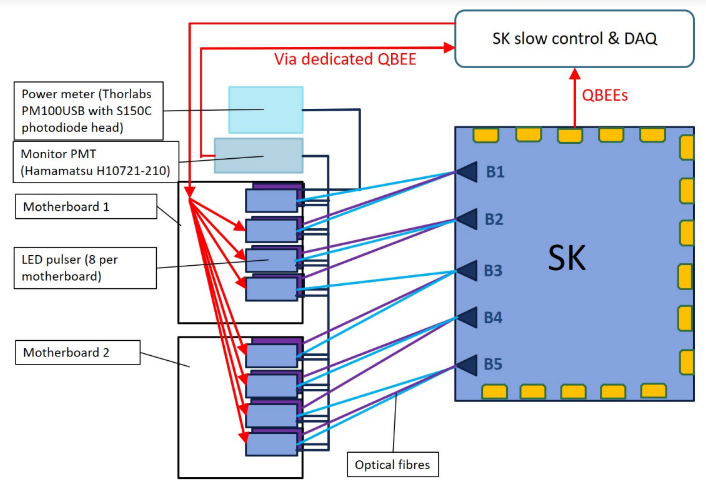
\includegraphics[width=0.8\textwidth]{Figures/ukli_system_architecture.png}
    \caption{UKLI electronics system architecture, showing optical fibre and motherboard couplings and QBEE connections.}
    \label{fig:ukli_system_architecture}
\end{figure}

The light being pulsed has a wavelength of 435 nm and is produced by light emitting diodes which are controlled by Field Programmable Gate Arrays and uses sixteen LED pulser boards placed on two motherboards (8 LED pulser boards on each) which controls which channel to send a signal to. Fifteen of the sixteen channels deliver light into the detector, while the remaining channel sends light to a seperate monitoring system. Each LED is coupled to three optical fibres, a channel connected to the monitor PMT, secondly to an optical fibre which sends light into the Super-Kamiokande detector, and to a spare. The monitor PMT is a 2 inch Hamamatsu PMT which has a peak sensitivity to 400 nm wavelength light. The monitor PMT is connected to one of the QBEE (QTC-based electronics with Ethernet) channels for the detector to record the monitoring signal into the data stream. 
\newline

The monitor PMT is installed inside a custom 3D printed box to make sure there is no external light reaching it. There are nineteen fibres input to the PMT, these are kept in place against the PMT's photocathode. There is one fibre for each of the sixteen LEDs and the last three channels are reserve. The channel which is coupled to the LED board for monitoring of the system is used to calibrate the monitor PMT, where the signal from this channel is inputted into the optical power meter.

\subsection{UKLI System Optics}

Unlike the Korean laser system mentioned in Chapter 4 that injects light into the detector using an optical fibre which has an opening angle of 4 degrees, the UK Light Injection system contains three different types of light injection optics, with each having a different opening angle: a bare fibre, a collimator and a diffuser. This range of optics can accomadate a larger variety of calibration measurements, and better suit the multiple applications of the light injection system, including it being better for monitoring purposes. 

\subsubsection{The Collimator Optic}

A 2-degree opening half angle is achieved by the collimator optic by using a graded index lens (GRIN) connected to a bare fibre optic cable - this GRIN lens reduces the opening angle of the light coming from the fibre optic. A schematic of the collimator design can be seen in Figure \ref{fig:collimator_schematic}. The GRIN lens is kept in position within the lens mount where a HAFC connector is drilled in to take a lens through the centre of the hole inside it, and there is a 2.35 mm diameter opening in front of the glass window in front of the GRIN lens in order to reduce background light which is not on-axis. All holes drilled into the collimator setup are filled with epoxy to prevent water from damaging the components. 

\begin{figure}
    \centering
    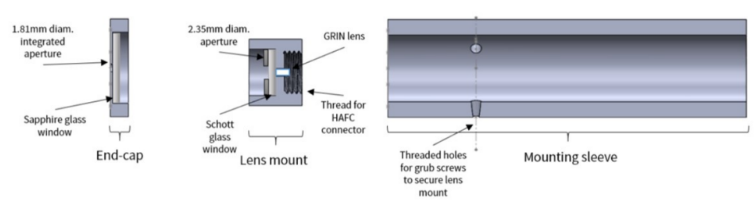
\includegraphics[width=0.8\textwidth]{Figures/collimator_schematic.png}
    \caption{Collimator schematic including the end-cap, lens mount and mounting sleeve structures.}
    \label{fig:collimator_schematic}
\end{figure}

Having such a confined beam allows for a very exact target position on the tank wall, and by decreasing the size of the target beam spot compared to the bare optical fibre, less hit PMTs outside of the target spot are excluded meaning that there are more hits in the water calibration data. Due to the fact that the very collimated beams mean that there is no overlap of beam spots, there can be measurements of the water scattering and absorption coefficients made that are position dependent, allowing for an observation of how the water parameters depend on depth in the tank. 

\subsubsection{The Diffuser Optic}

The diffuser optic is a wide angled beam with a opening half-angle of 40 degrees. It allows for water coefficient measurement calibration and light attenuation length in water. The diffuser optic is made of a Poly(methyl methacrylate) (PMMA) ball which is a piece of acrylic resin in the shape of a half sphere and it contains PMMA particles suspended in silicone gel, similar to the design of the ``laserball'' used to calibrate the SNO+ detector \cite{Moffat_2005}. As a result of this, the mean free path of light that is injected into the center of the diffuser ball is much shorter than the radius of the ball, so each photon scatters many times off the PMMA particles at random so that the exiting angle of the light is also random. This randomised exit direction of the photons means that the beam timing and intensity would be uniform.  
\newline
 Figure \ref{fig:diffuser_photo} shows a photograph of one of the diffusers used, and one of the diffuser ball enclosures. The enclosure is made of high grade stainless steel and using a chemical and water resistant epoxy resin, all the components were ensured to be watertight. 

\begin{figure}
    \centering
    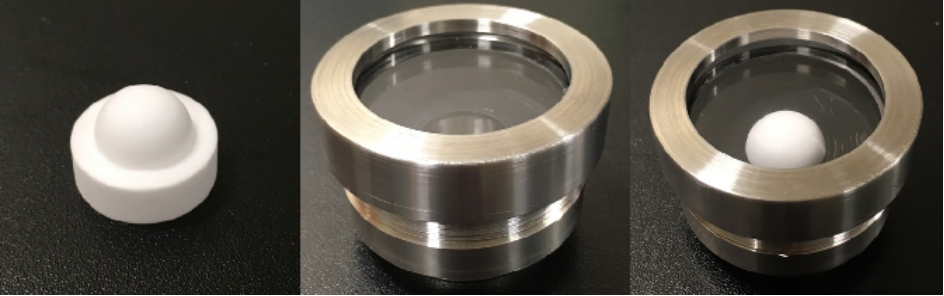
\includegraphics[width=0.7\textwidth]{Figures/diffuser_photo.png}
    \caption{Photograph of the diffuser by itself (left), empty diffuser enclosure (centre) and diffuser inside enclosure (right).}
    \label{fig:diffuser_photo}
\end{figure}

\subsubsection{Bare Fibre and Optical Plate}

The bare fibre injector are 1 mm step index fibres, and are approximately 20 cm in length and are used for validation purposes with the bare fibres in the Korean optical calibration system. These short fibres are screwed into the back end of the optical plate that the collimator and diffuser optics are mounted on.


\subsubsection{Results of optics test stands}

In order to test the collimator and diffuser optics, scans of the angular distributions were made using diffuser and collimator test-stands. These scans would show angular distributions of the light intensity, and details of the setup of each test stand are given here. For the diffuser test-stand the angular distribution of the light output was captured using the setup shown in Figure \ref{fig:diffuser_test_stand}. A birds-eye view schematic of the setup is shown in Figure \ref{fig:schematic_dif}.

\begin{figure}
    \centering
    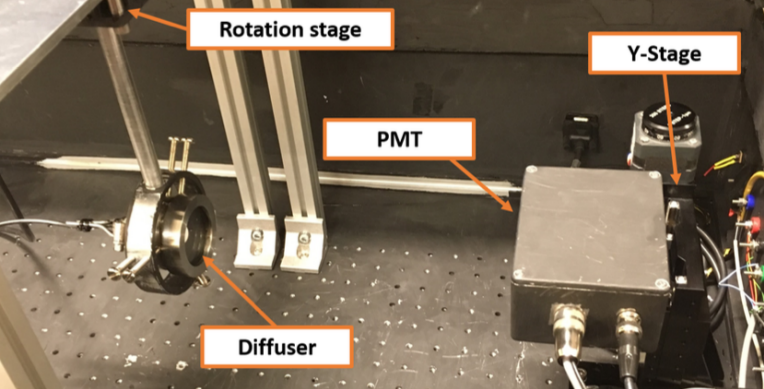
\includegraphics[width=0.7\textwidth]{Figures/diffuser_test_stand.png}
    \caption{Setup of the diffuser test stand provided by Warwick University}
    \label{fig:diffuser_test_stand}
\end{figure}


The test stand setup for the diffuser optics consists of a test diffuser ball placed inside a diffuser enclosure, a rotation stage which allows for the movement of the diffuser between -40 and 40 degrees, and a PMT used for pulse intensity measurement set up 250 mm away from the diffuser. An optical fibre couples the diffuser under test to a laser set to a wavelength of 450 nm. 

The setup for the collimator test stand at the University of Warwick is shown in Figure \ref{fig:coll_test_stand}.  The setup for the collimator optic captures the beam cross section by moving a CMOS camera along the beam direction. 

\begin{figure}
    \centering
    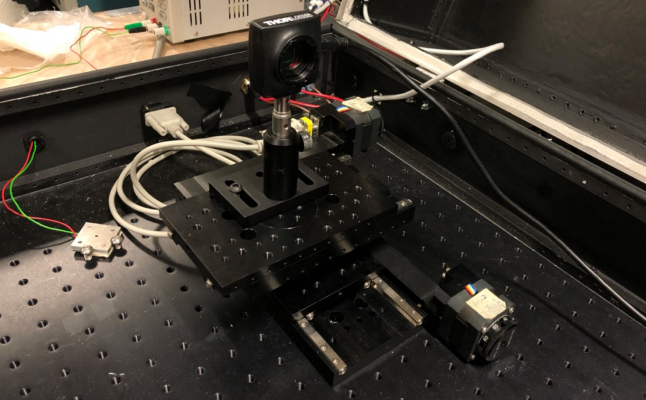
\includegraphics[width=0.7\textwidth]{Figures/coll_test_stand.png}
    \caption{Setup of the collimator test stand provided by Warwick University}
    \label{fig:coll_test_stand}
\end{figure}

Figure \ref{fig:diffuser_TF1} shows distributions provided by this test stand data which are preliminary TF1 fits made by ROOT to the light profiles for the diffuser.  The x-axis scale shows the polar angle the rotation stand moves through, while the y-axis scale shows the average of the integrated area under all the pulses recorded by the PMT and is not normalised. 

\begin{figure}[!htbp]
    \centering
    
    \caption{Light profiles for the diffuser optics provided by The University of Warwick}\label{fig:diffuser_TF1}
    
    \subfloat[]{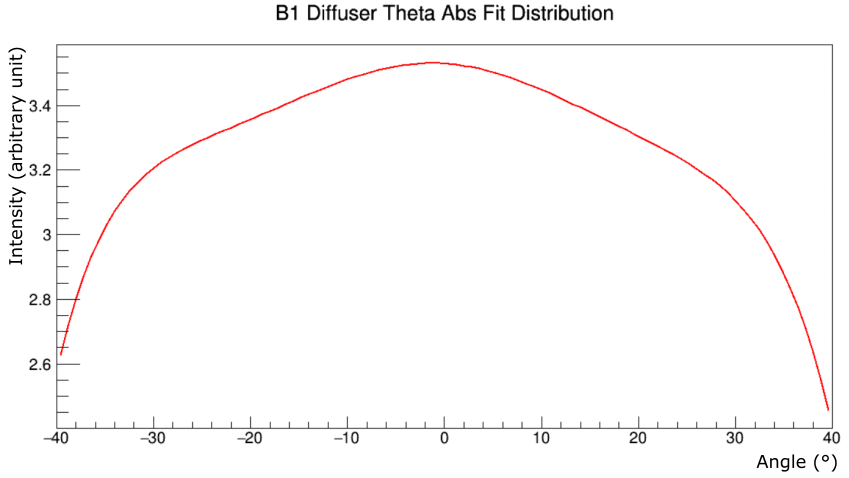
\includegraphics[width=0.33\textwidth]{Figures/B1_diffuser_fit.PNG}}\hfill
    \subfloat[]{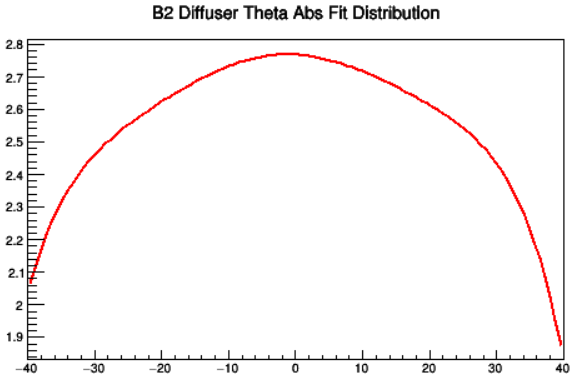
\includegraphics[width=0.33\textwidth]{Figures/B2_diffuser_fit.PNG}}\hfill
    \subfloat[]{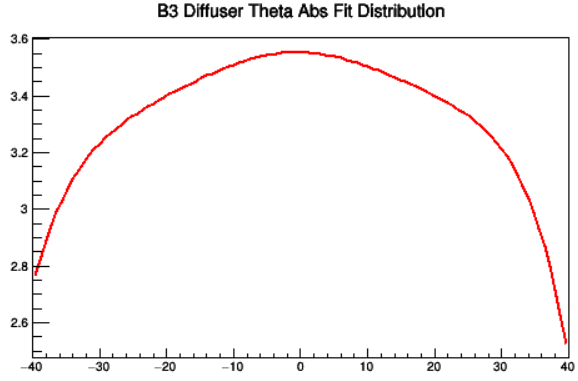
\includegraphics[width=0.33\textwidth]{Figures/B3_diffuser_fit.PNG}}
    
    \subfloat[]{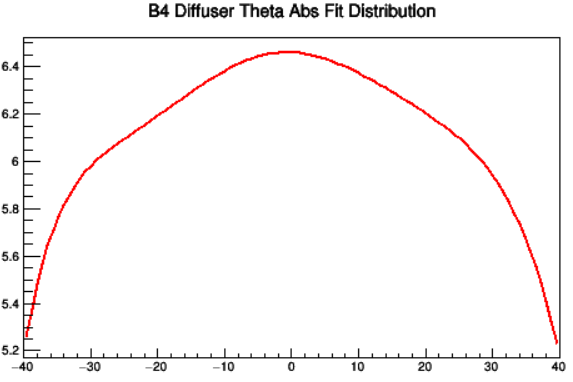
\includegraphics[width=0.33\textwidth]{Figures/B4_diffuser_fit.PNG}}%
    \hspace*{0.005\textwidth}%
    \subfloat[]{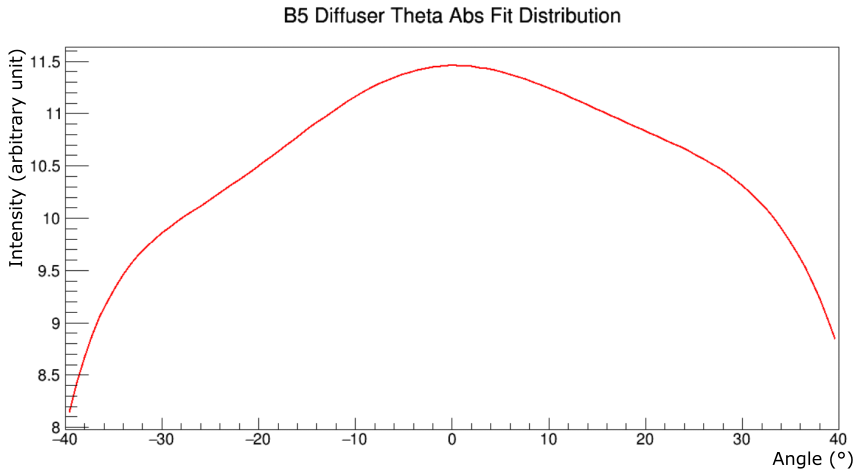
\includegraphics[width=0.33\textwidth]{Figures/B5_diffuser_fit.PNG}}
    
\end{figure}

Figure \ref{fig:collimator_TF1} shows TF1 fits made by ROOT to the light profiles for the collimator. The angular distributions shown give the distribution of the polar angle in degrees of light intensity which are relative to the virtual position from which the light cone originates, averaged over all the orientations of the azimuthal angle. 

\begin{figure}[!htbp]
    \centering
    
    \caption{Light profiles for the collimator optics provided by The University of Warwick}\label{fig:collimator_TF1}
    
    \subfloat[]{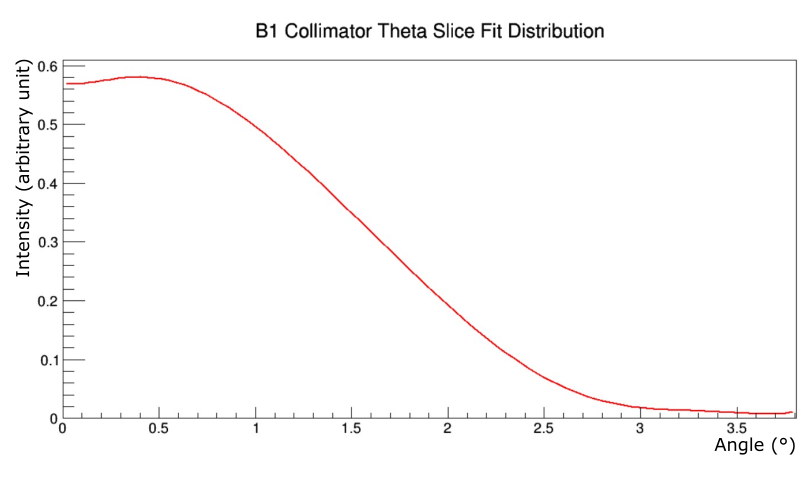
\includegraphics[width=0.33\textwidth]{Figures/B1_collimator_fit.PNG}}\hfill
    \subfloat[]{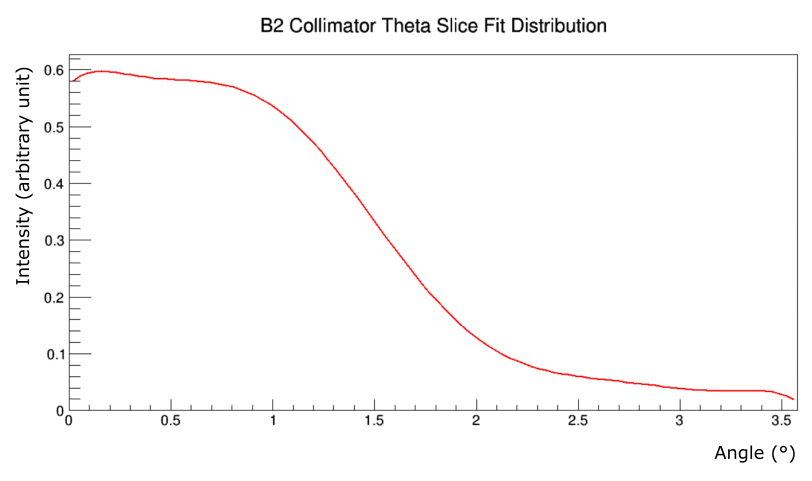
\includegraphics[width=0.33\textwidth]{Figures/B2_collimator_fit.PNG}}\hfill
    \subfloat[]{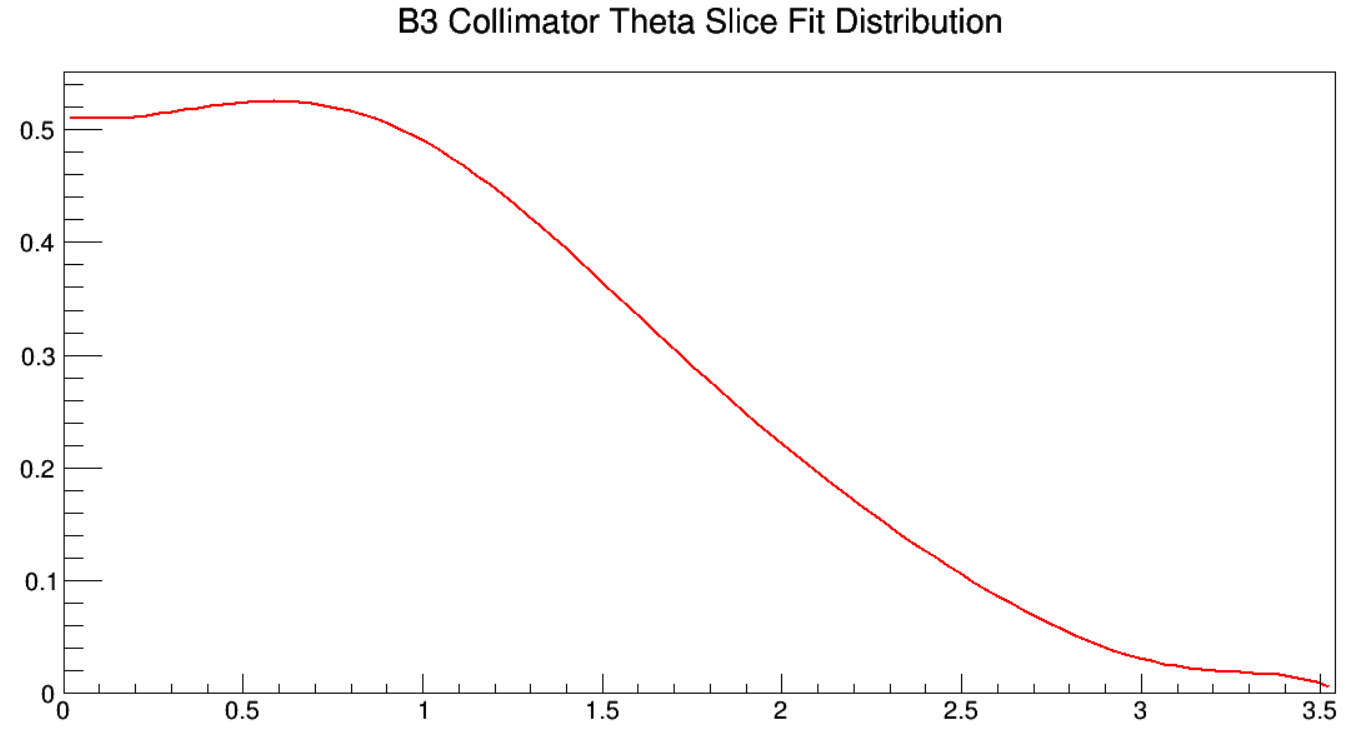
\includegraphics[width=0.33\textwidth]{Figures/B3_collimator_fit.PNG}}
    
    \subfloat[]{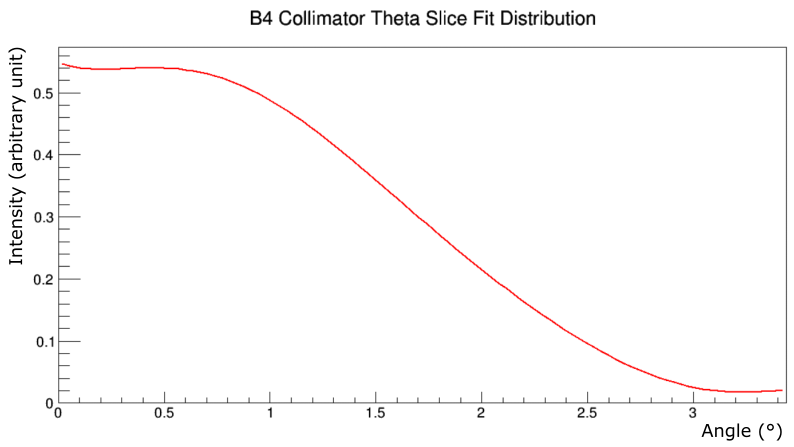
\includegraphics[width=0.33\textwidth]{Figures/B4_collimator_fit.PNG}}%
    \hspace*{0.005\textwidth}%
    \subfloat[]{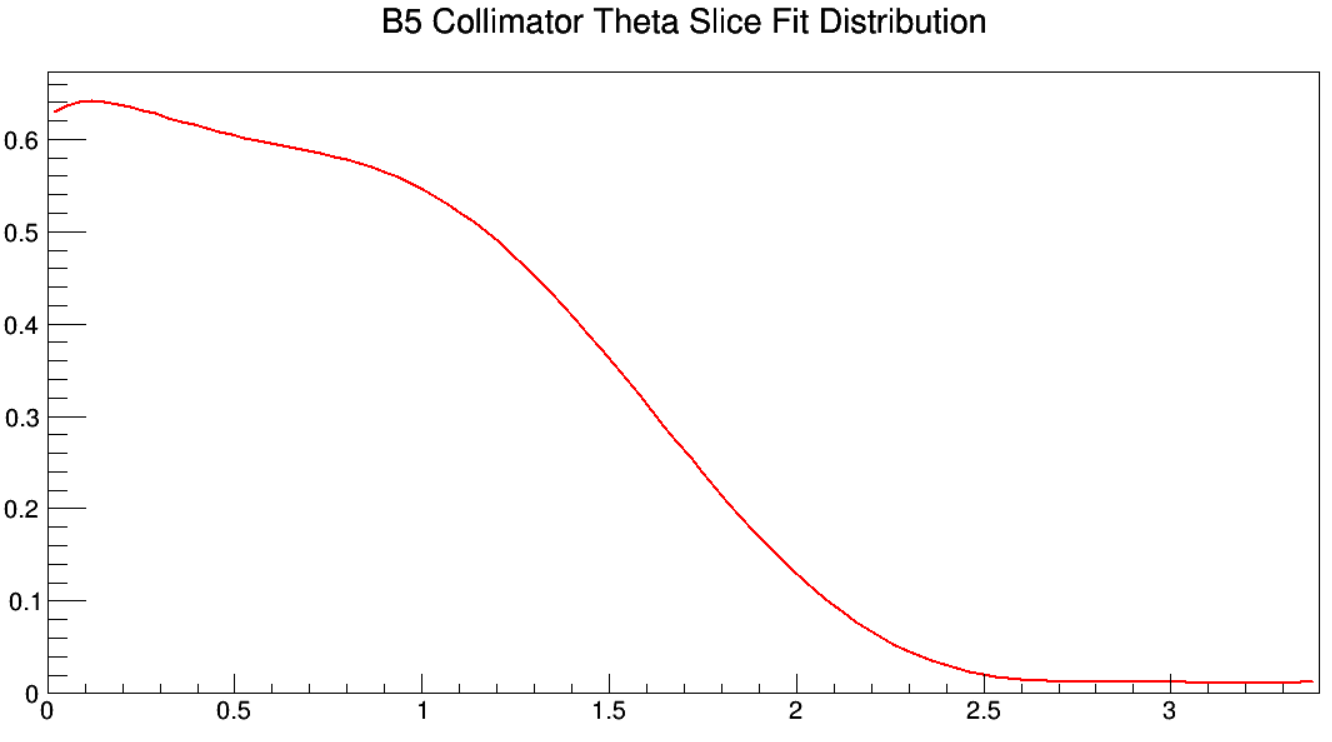
\includegraphics[width=0.33\textwidth]{Figures/B5_collimator_fit.PNG}}
    
\end{figure}

\subsubsection{UK Calibration data}

In September of 2019 and November of 2019 two sets of test data were taken of the collimator, the diffuser and the bare fibre optic (the B2 bare fibre). For the September 2019 data, all of the data for the B1-B5 optics was taken with 100,000 events, however due to the B3 and B5 collimator from the September 2019 data showing a very weak signal, 150,000 events were taken with the B3 collimator data and 200,000 events were taken with the November 2019 data. Using an event display developed by the University of Warwick, occupancy plots of the test data sets were produced. Figure \ref{fig:occupancy_coll} shows the occupancy plots for the collimator optic from the November 2019 dataset showing the beam spot inside the unrolled volume of the Super-Kamiokande detector. Similarly, Figure \ref{fig:occupancy_diffuser} shows the occupancy plots for the diffuser optic from the November 2019 dataset. The graph in the bottom right hand corner of the occupancy plots show the corrected time-of-flight plots for the PMT hits from the injector. 

\begin{figure}[!htbp]
    \centering
    
    \caption{Occupancy plot for the collimator optics from the UKLI November 2019 test run} \label{fig:occupancy_coll} 
    
    \subfloat[]{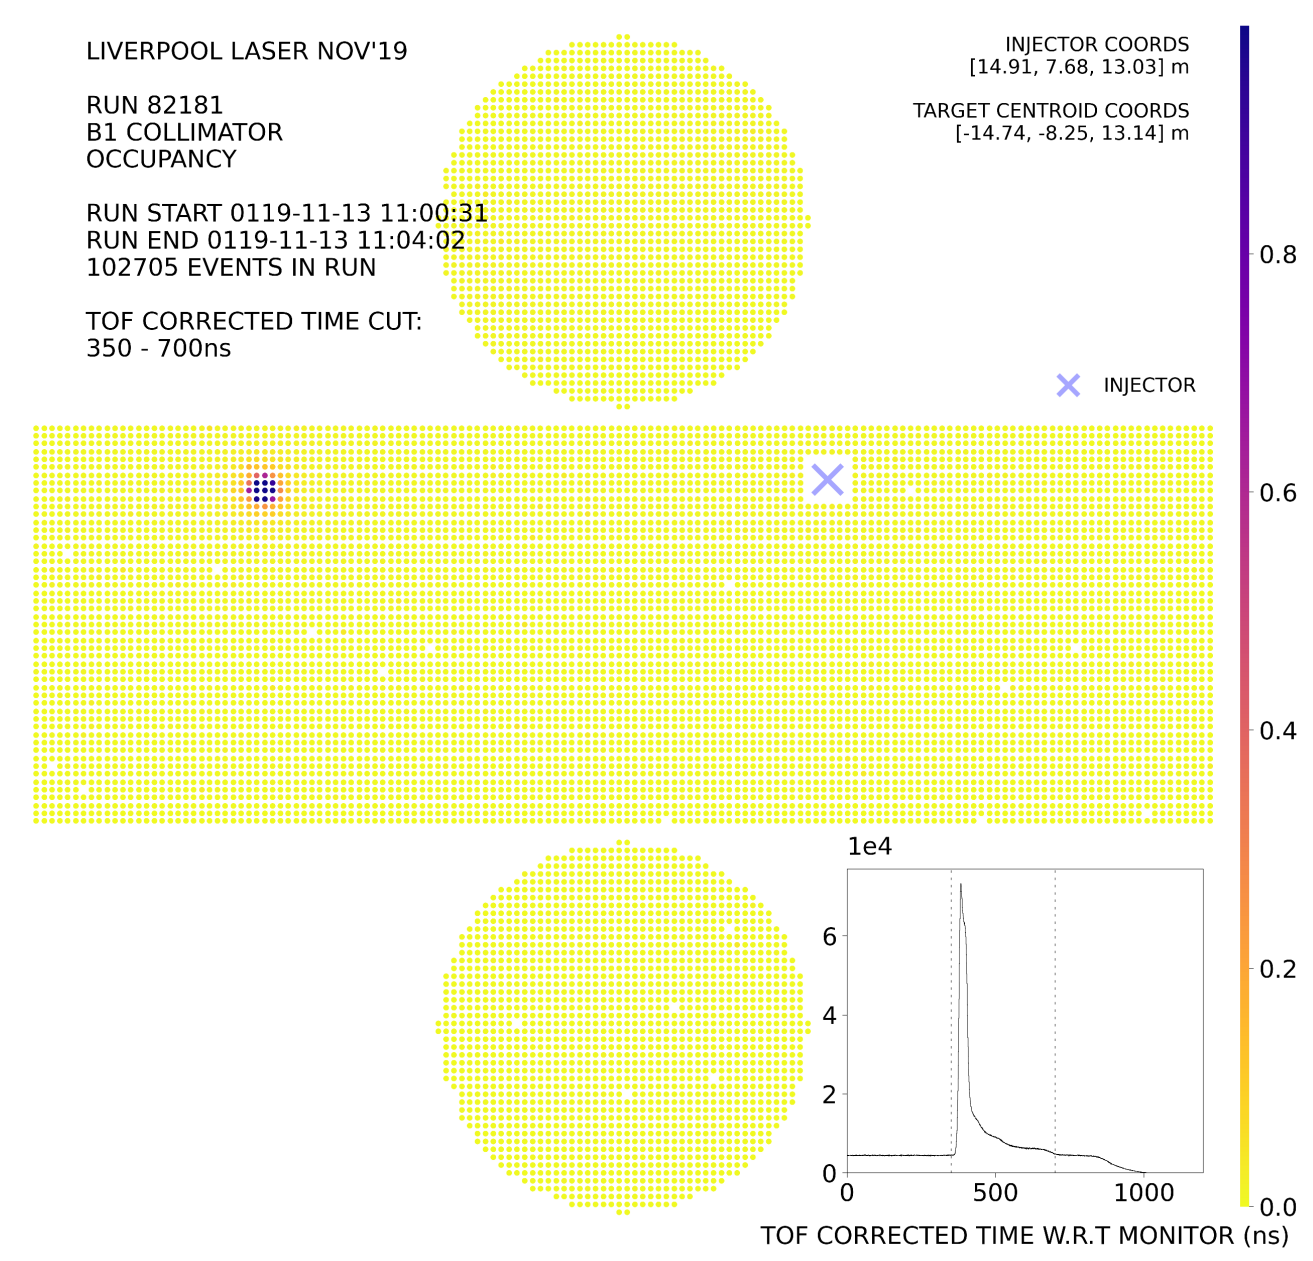
\includegraphics[width=0.49\textwidth]{Figures/B1_occupancy_coll.PNG}} \hfill
    \subfloat[]{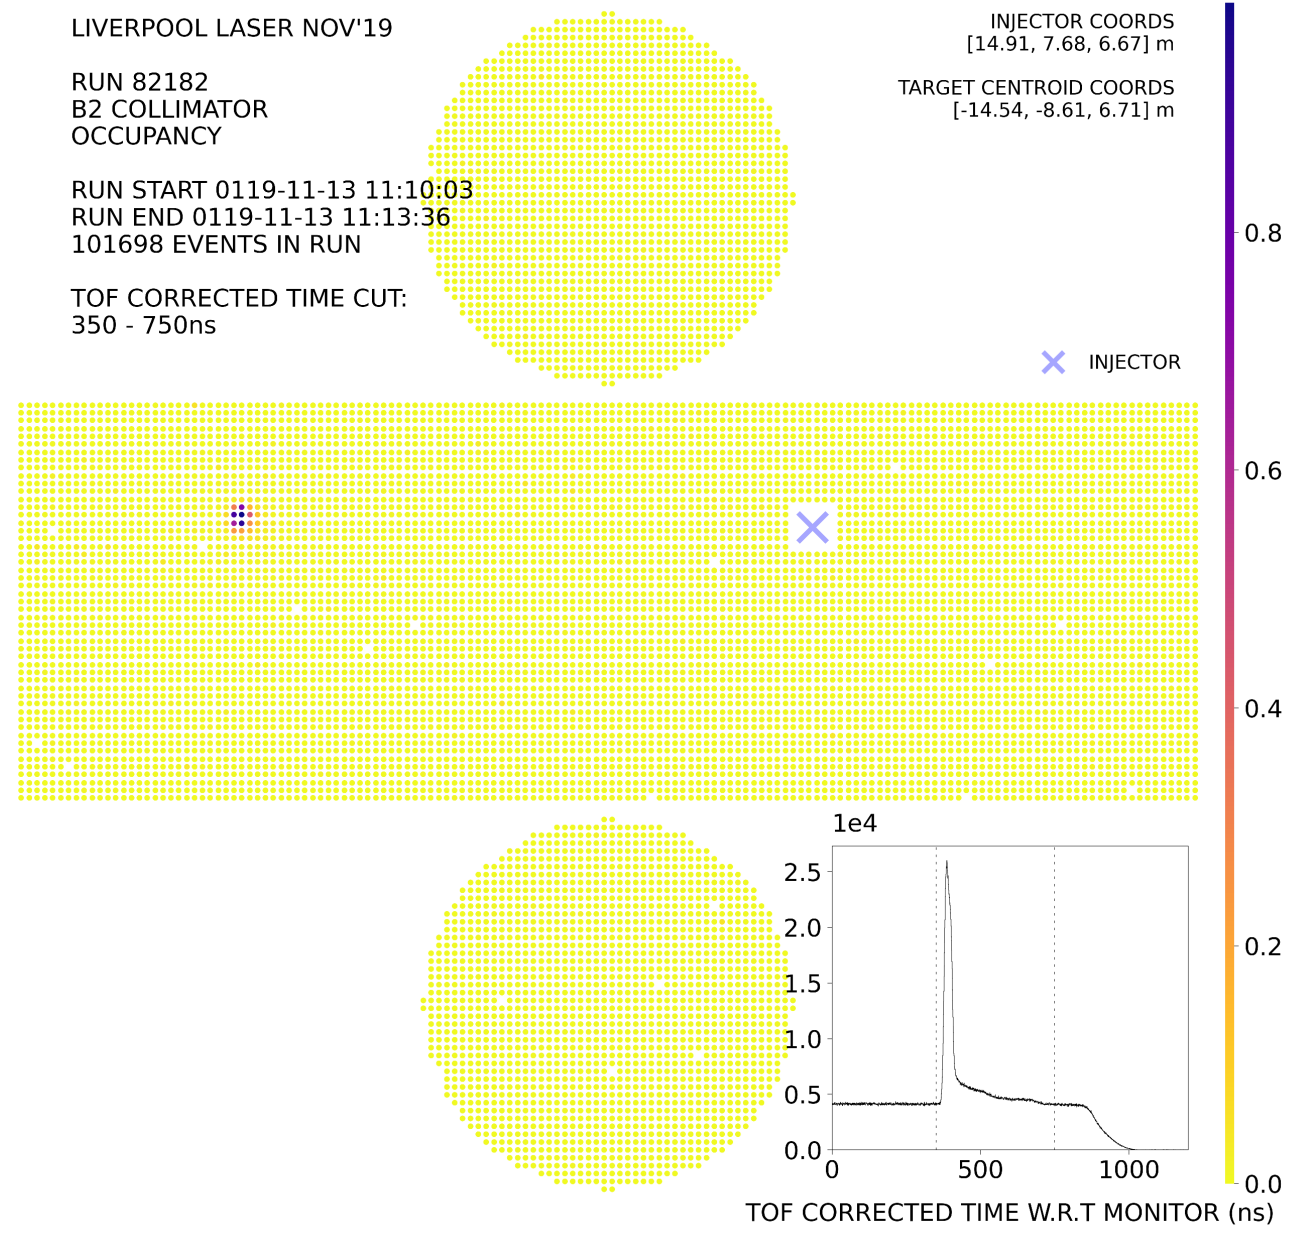
\includegraphics[width=0.49\textwidth]{Figures/B2_occupancy_coll.PNG}} \par
    \subfloat[]{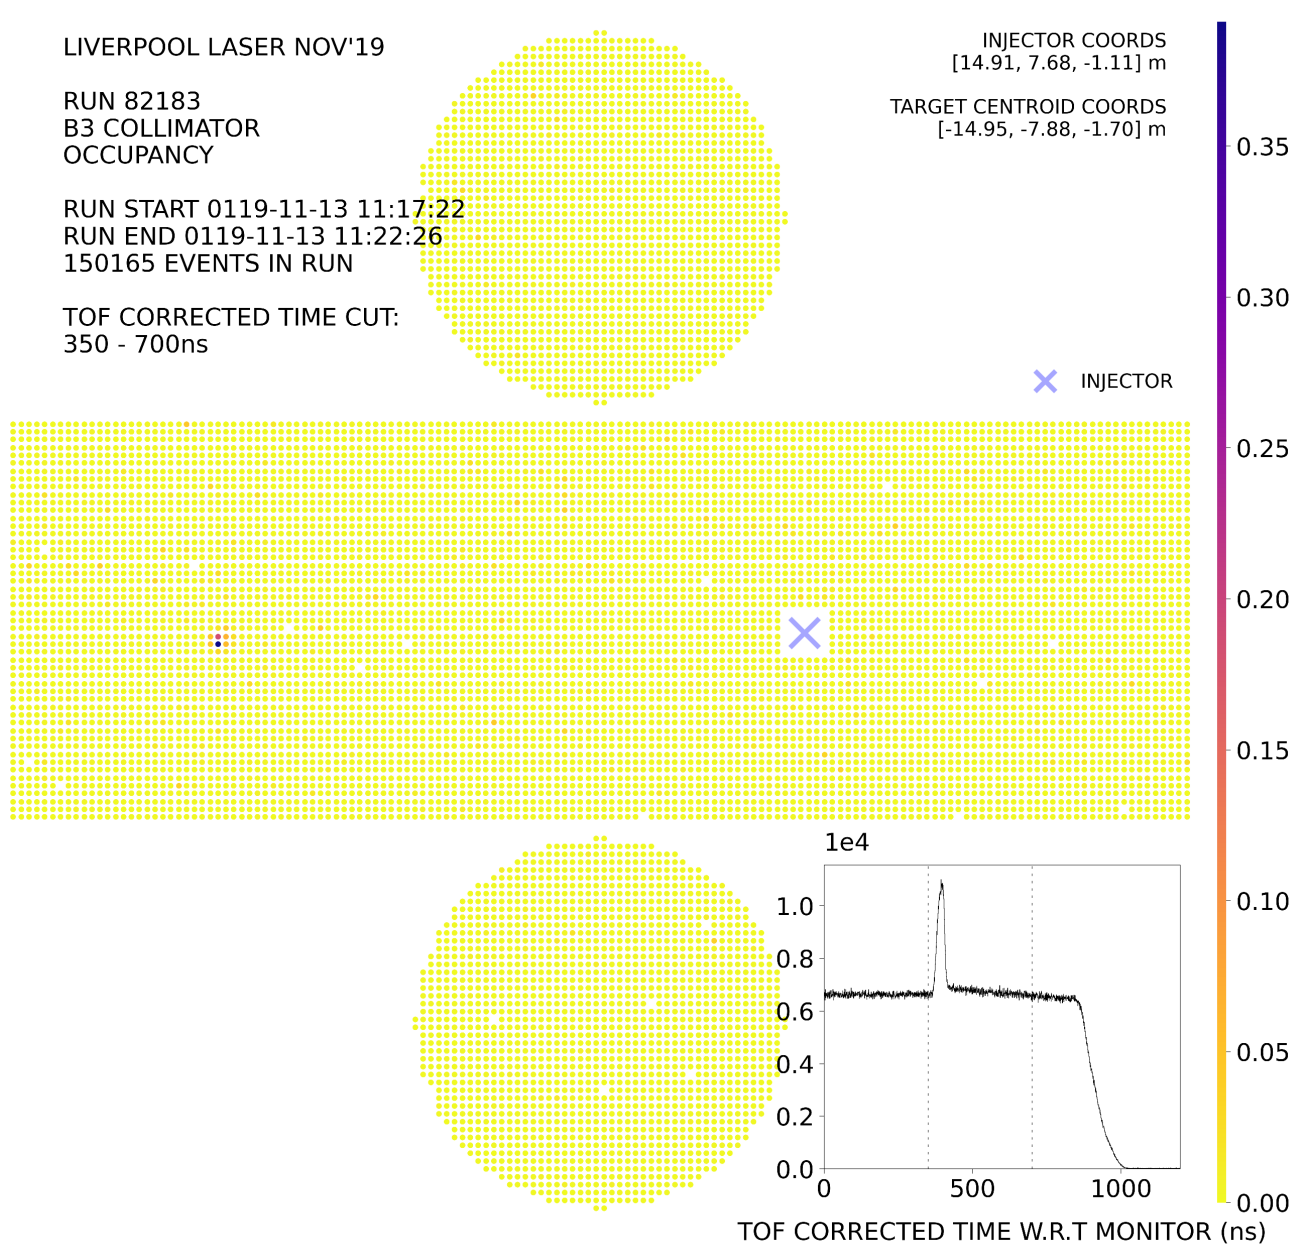
\includegraphics[width=0.49\textwidth]{Figures/B3_occupancy_coll.PNG}} \hfill
    \subfloat[]{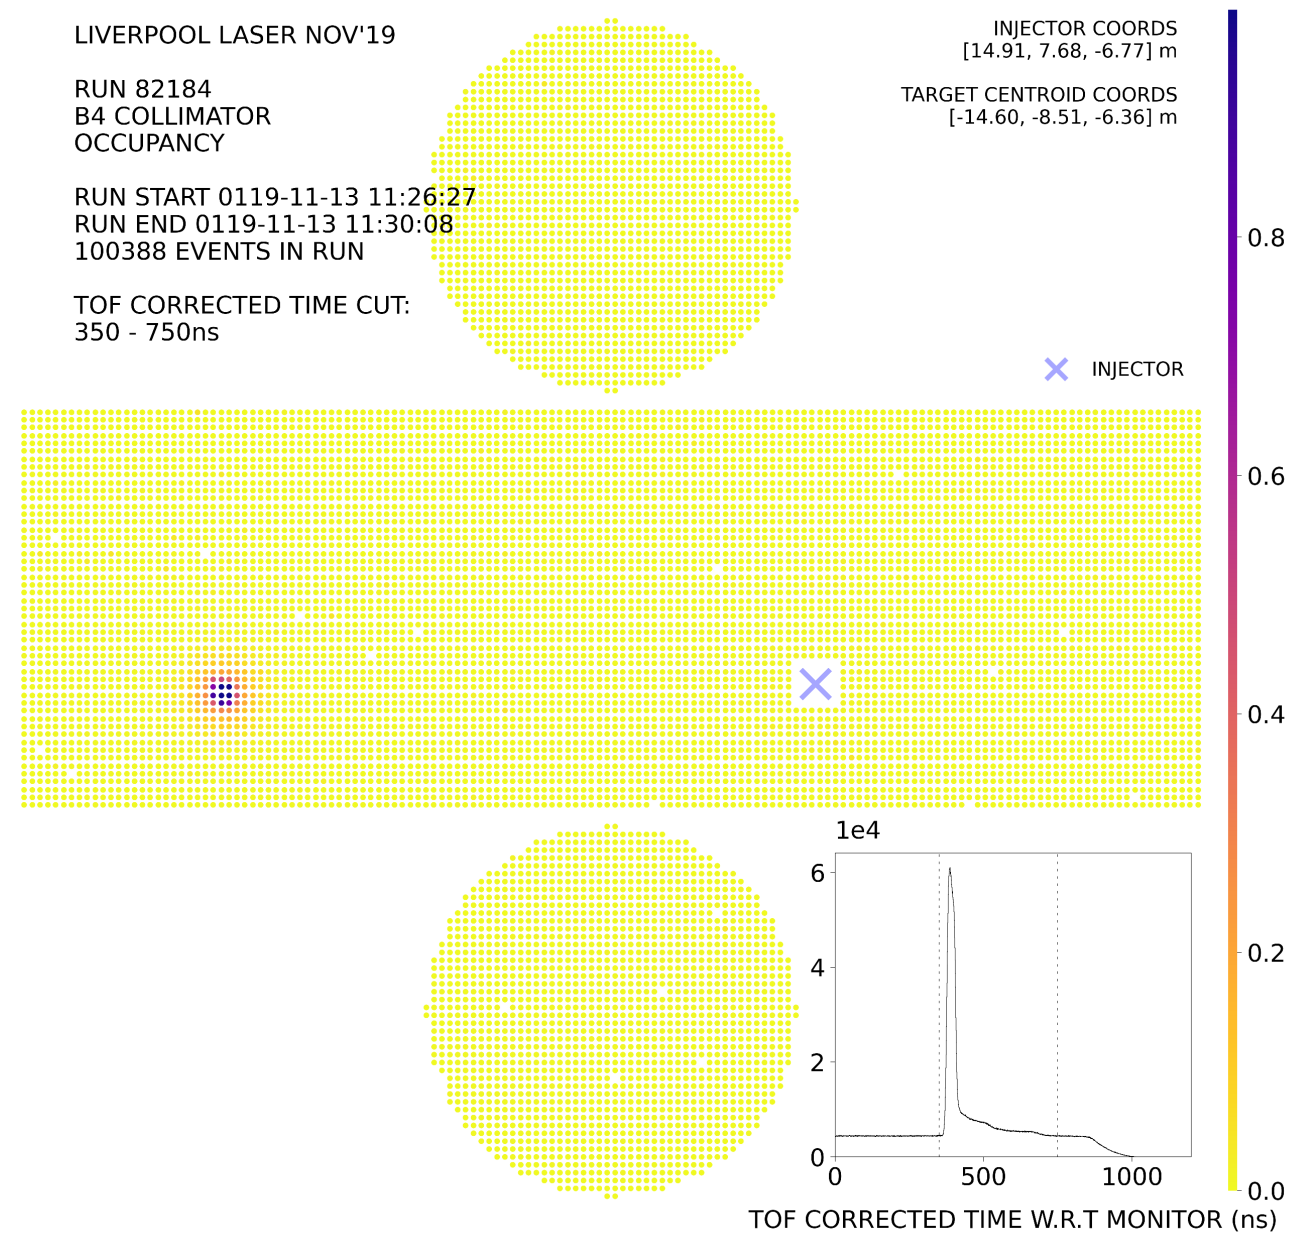
\includegraphics[width=0.49\textwidth]{Figures/B4_occupancy_coll.PNG}} \par
    \subfloat[]{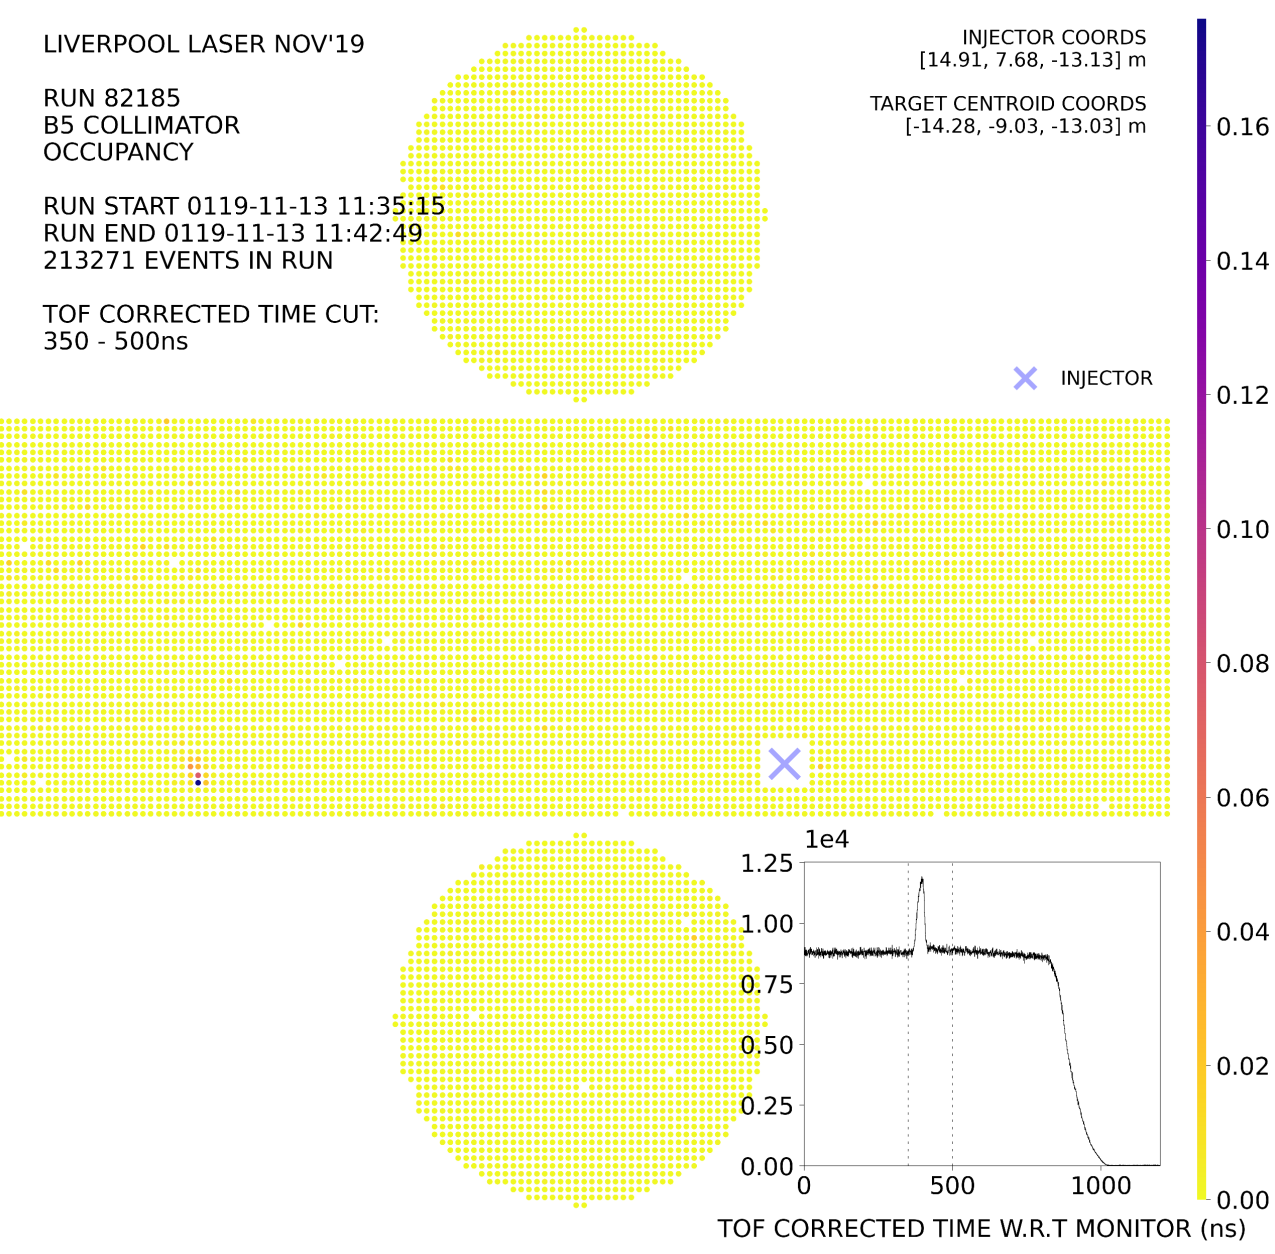
\includegraphics[width=0.49\textwidth]{Figures/B5_occupancy_coll.PNG}}
    
\end{figure}

\begin{figure}[!htbp]
    \centering
    
    \caption{Occupancy plot for the diffuser optics from the UKLI November 2019 test run} \label{fig:occupancy_diffuser} 
    
    \subfloat[]{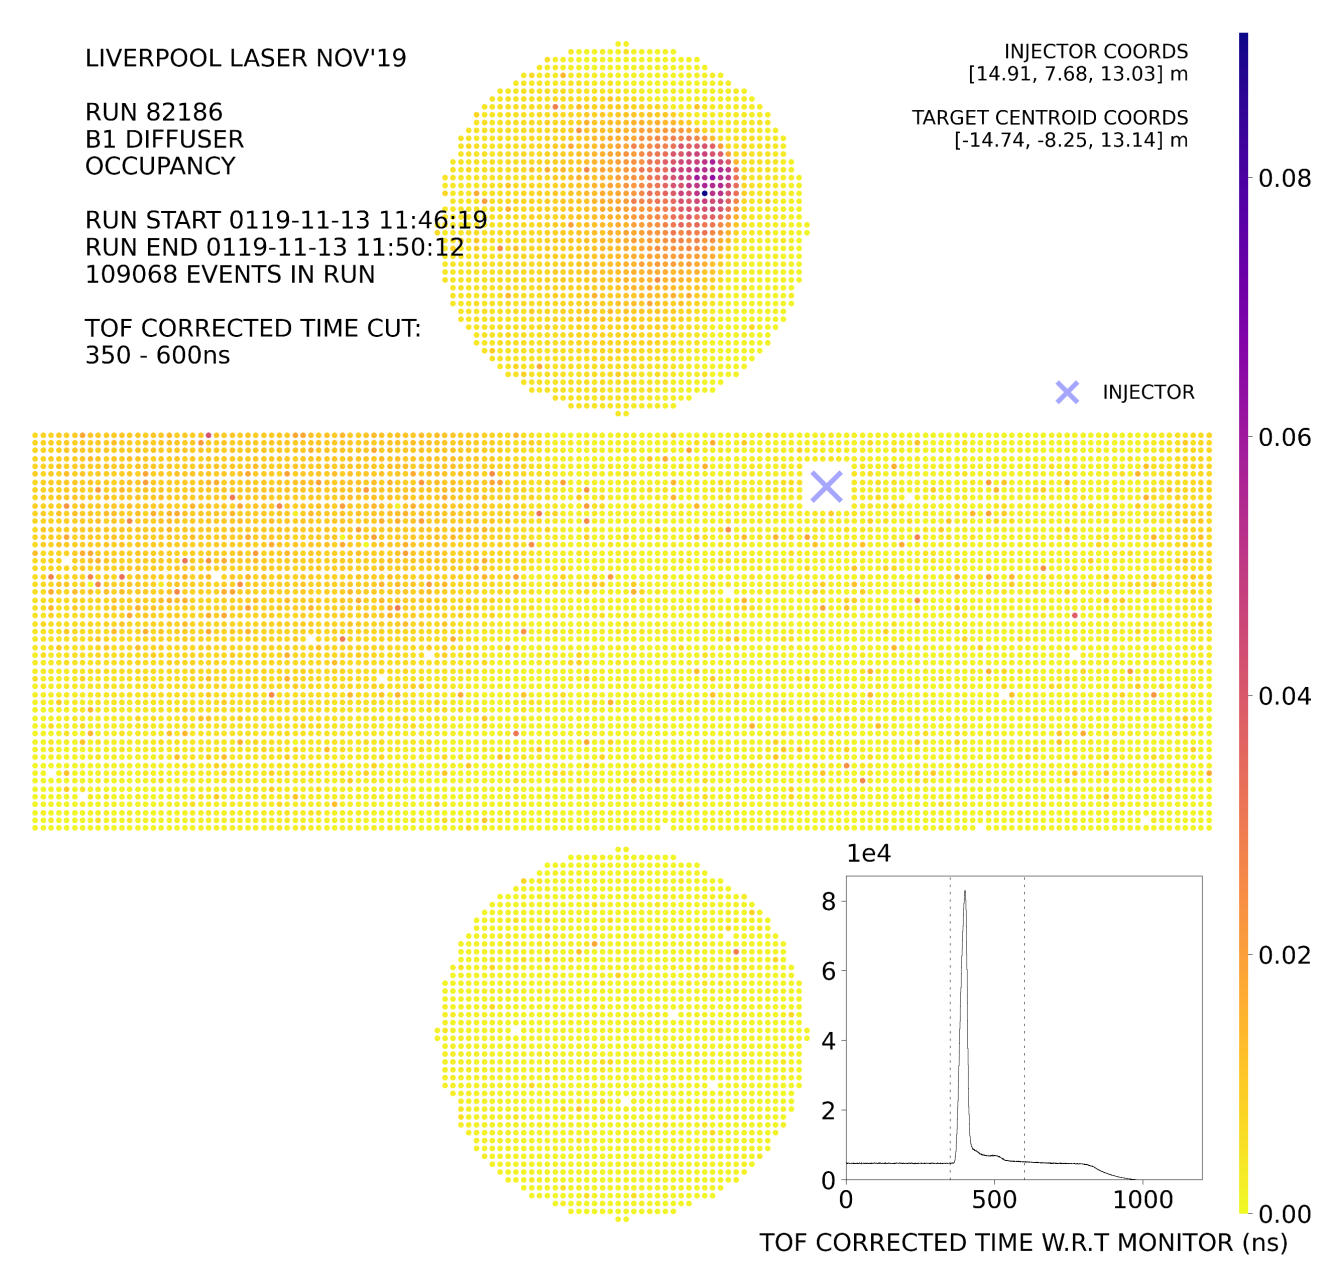
\includegraphics[width=0.49\textwidth]{Figures/B1_occupancy_diff.PNG}} \hfill
    \subfloat[]{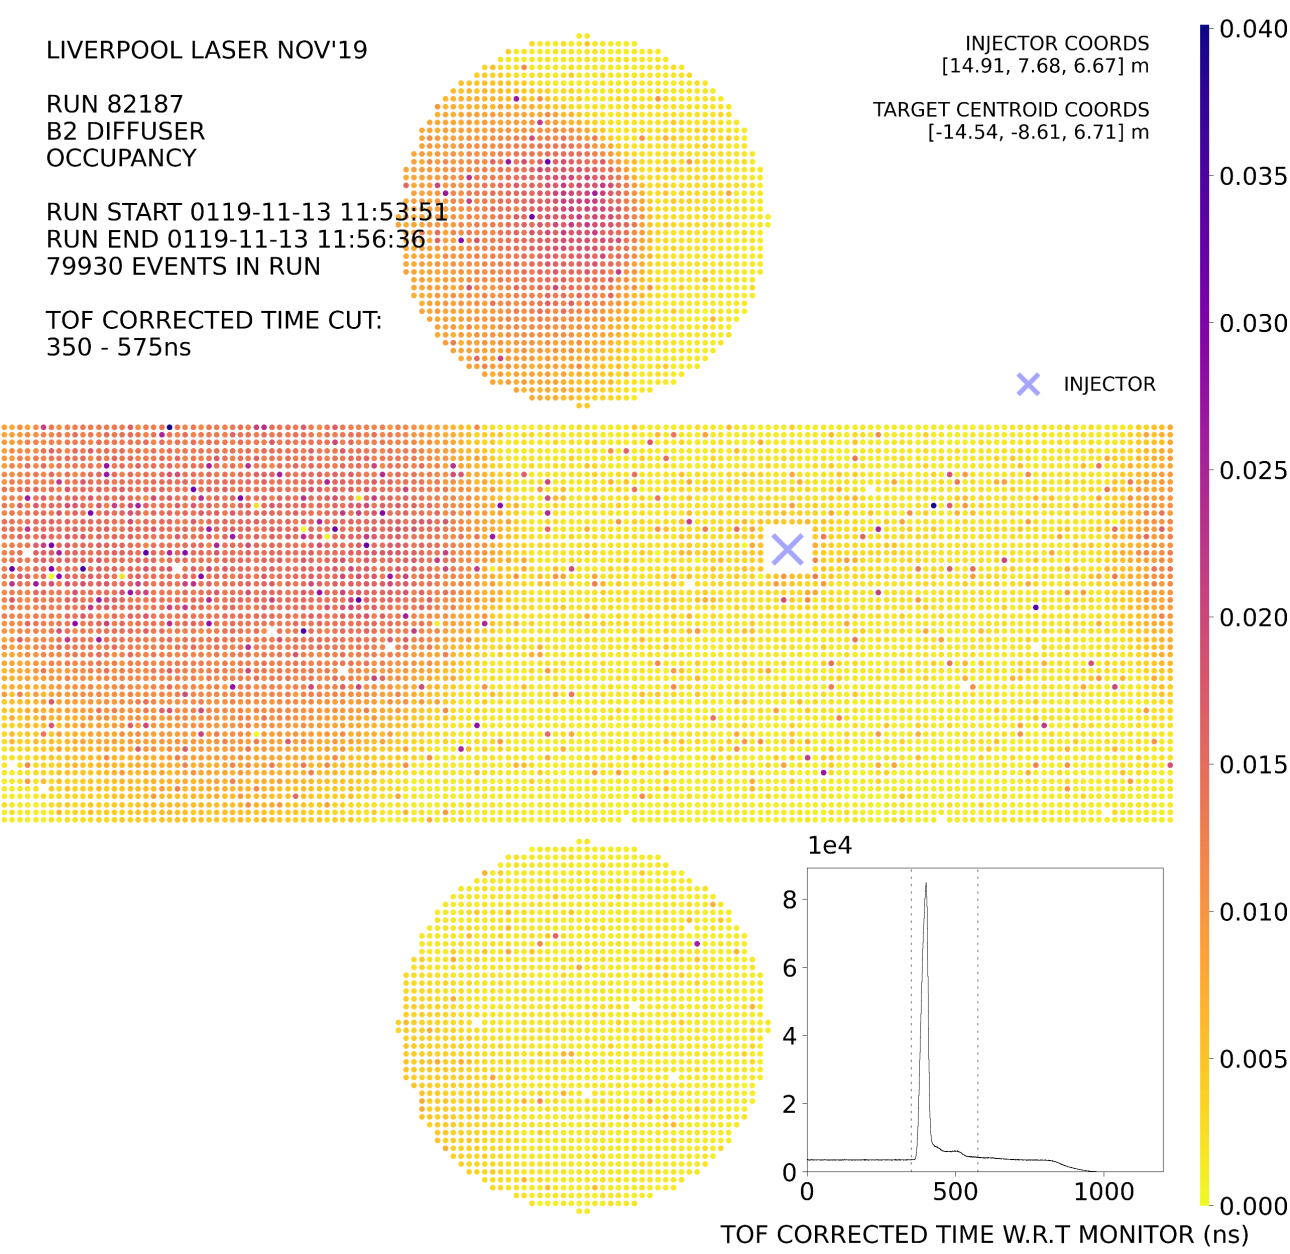
\includegraphics[width=0.49\textwidth]{Figures/B2_occupancy_diff.PNG}} \par
    \subfloat[]{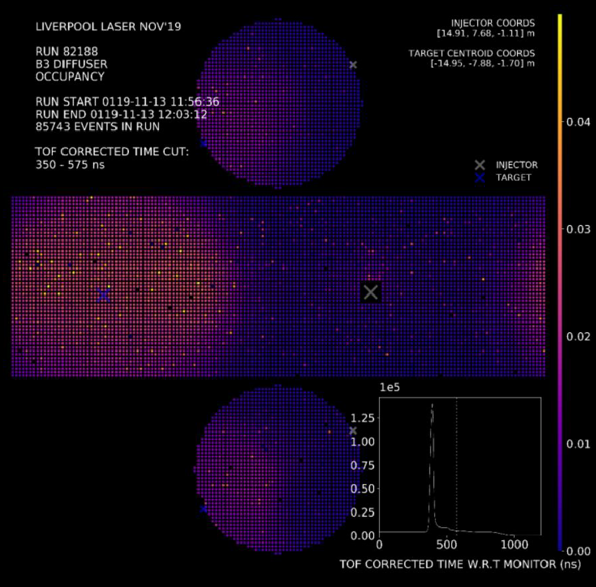
\includegraphics[width=0.49\textwidth]{Figures/B3_occupancy_diff.PNG}} \hfill
    \subfloat[]{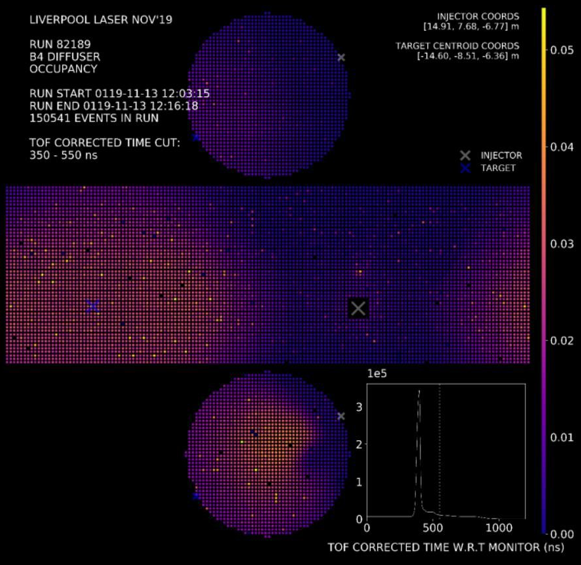
\includegraphics[width=0.49\textwidth]{Figures/B4_occupancy_diff.PNG}} \par
    \subfloat[]{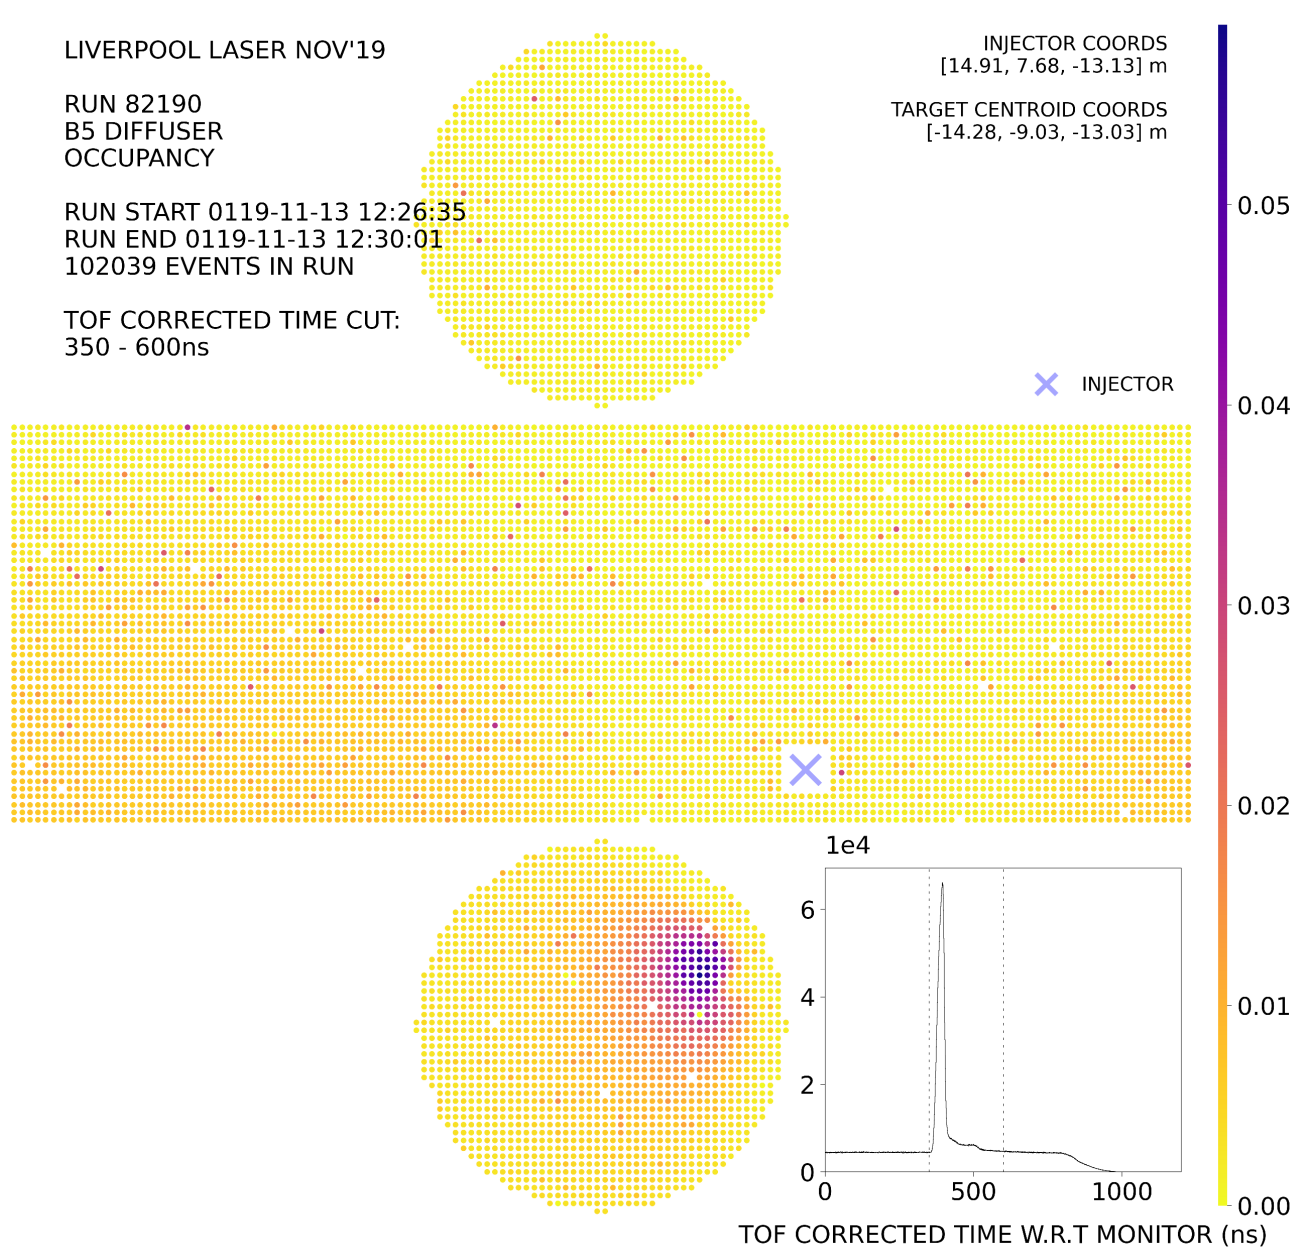
\includegraphics[width=0.49\textwidth]{Figures/B5_occupancy_diff.PNG}}
    
\end{figure}

In addition to test data being taken, there is also an ``autocalib'' system used for long term monitoring of the water parameters in Super-Kamiokande by the Korean laser system. In early 2020 the autocalib scheduler was modified to incorporate data taking by the UKLI system which was very useful for Gadolinium loading calibration purposes but also in the longer term, it will be useful in the monitoring of daily/weekly water coefficient property measurements, investigation of depth dependence with respect to the water properties and PMT property calibration. Figure \ref{fig:autocalib} shows the schedule for autocalib, and the black dashed lines show the position of the UK barrel collimator and diffusers with respect to the other autocalib data taking streams. The horizontal blue line shows the length of the one autocalib cycle, which is about 4.6 seconds, with each UKLI optic taking about 3310 events per day.

\begin{figure}
    \centering
    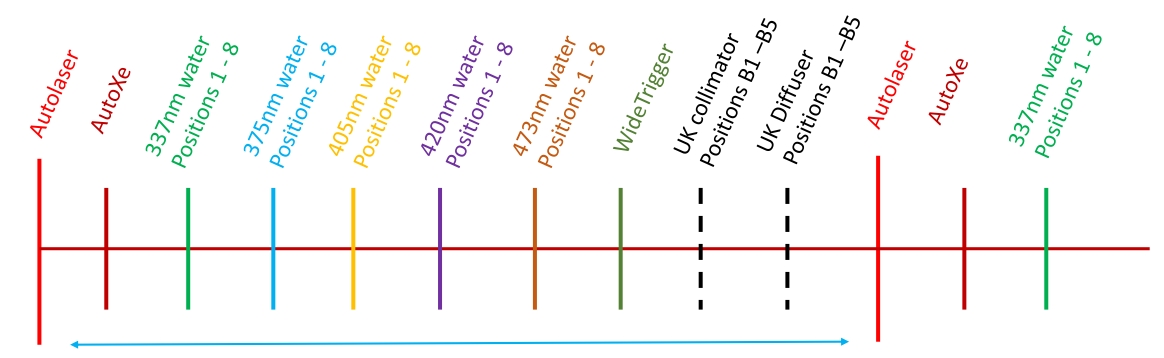
\includegraphics[width=0.8\textwidth]{Figures/autocalib.png}
    \caption{Schematic showing position of the UKLI in autocalib scheduler: the black dashed lines show the UKLI B1-B5 collimator and diffuser optics and the horizontal blue line shows the length of one autocalib cycle.}
    \label{fig:autocalib}
\end{figure}

Figures \ref{fig:occupancy_coll_auto} and \ref{fig:occupancy_diff_auto} shows the occupancy plots for autocalib data taken in July 2020: as can be seen in the text in the upper left hand corner, the number of events in the run is a lot less than the 100,000 events or so taken in the test runs, however they are more than sufficient for monitoring purposes.

\begin{figure}[!htbp]
    \centering
    
    \caption{Occupancy plot for the collimator optics from the UKLI Autocalib July 2020 run} \label{fig:occupancy_coll_auto} 
    
    \subfloat[]{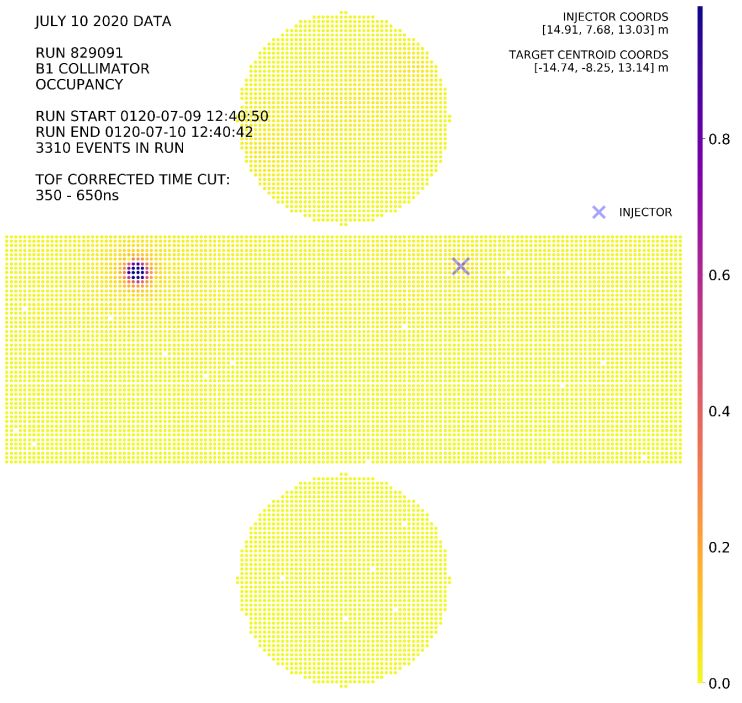
\includegraphics[width=0.49\textwidth]{Figures/B1_occupancy_coll_auto.PNG}} \hfill
    \subfloat[]{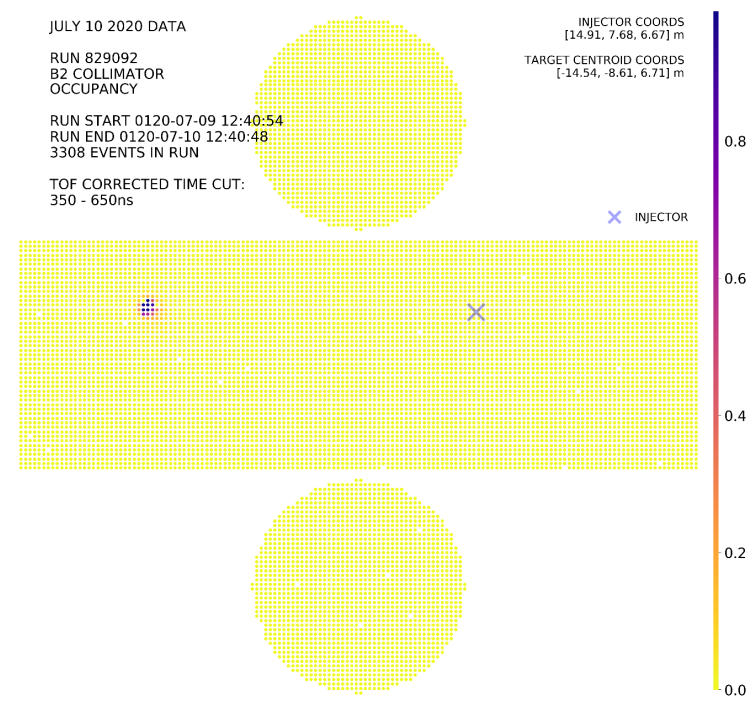
\includegraphics[width=0.49\textwidth]{Figures/B2_occupancy_coll_auto.PNG}} \par
    \subfloat[]{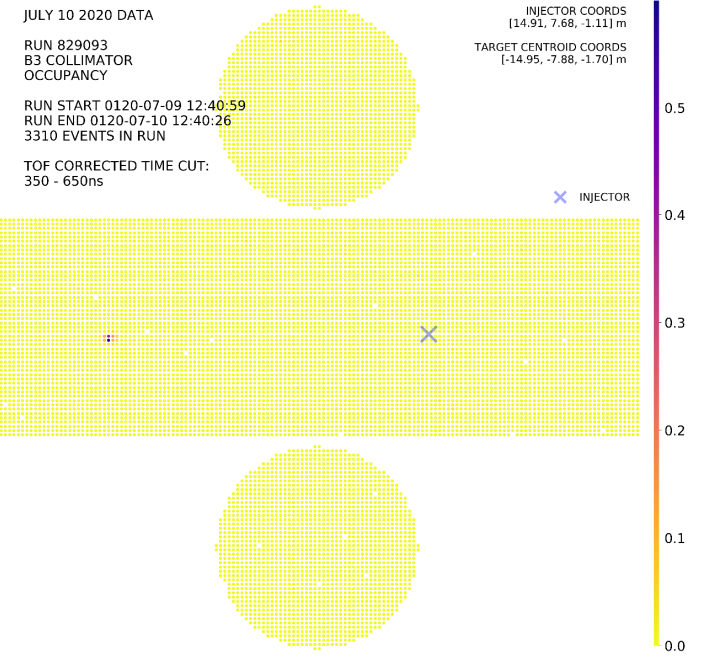
\includegraphics[width=0.49\textwidth]{Figures/B3_occupancy_coll_auto.PNG}} \hfill
    \subfloat[]{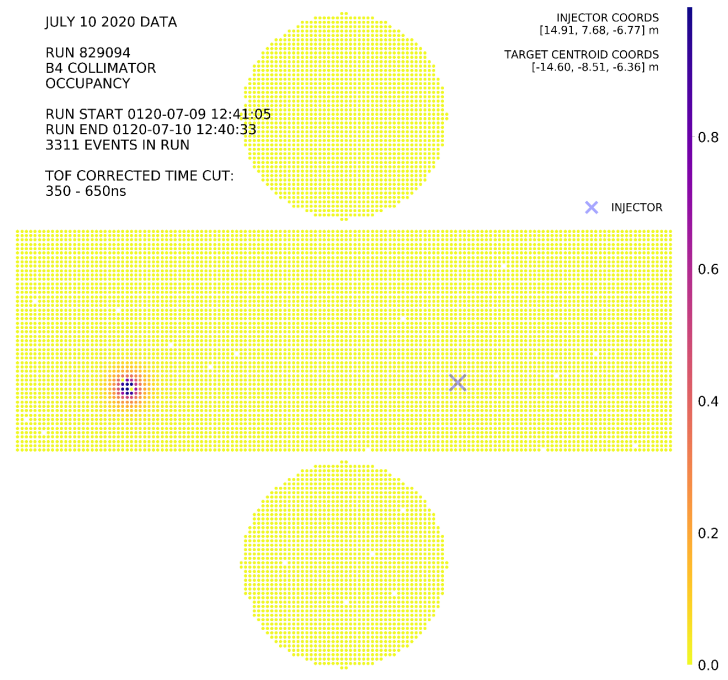
\includegraphics[width=0.49\textwidth]{Figures/B4_occupancy_coll_auto.PNG}} \par
    \subfloat[]{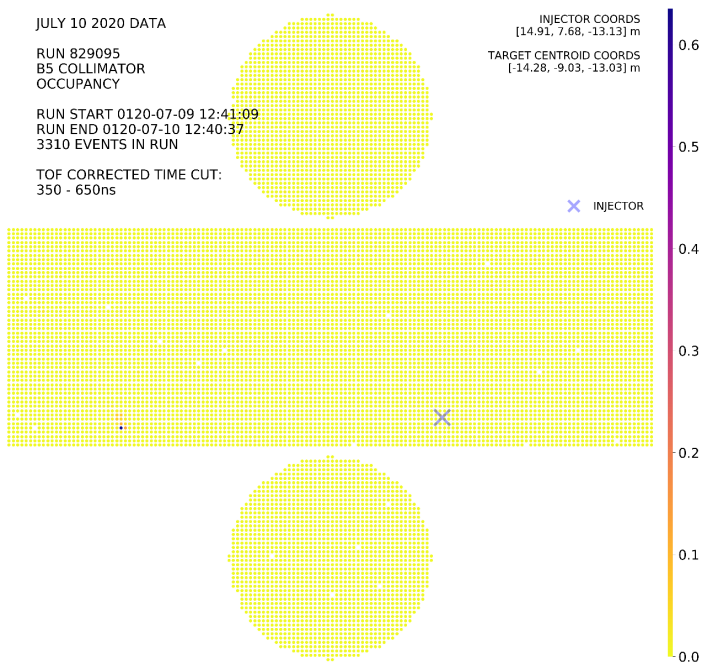
\includegraphics[width=0.49\textwidth]{Figures/B5_occupancy_coll_auto.PNG}}
    
\end{figure}

\begin{figure}[!htbp]
    \centering
    
    \caption{Occupancy plot for the diffuser optics from the UKLI Autocalib July 2020 run} \label{fig:occupancy_diff_auto} 
    
    \subfloat[]{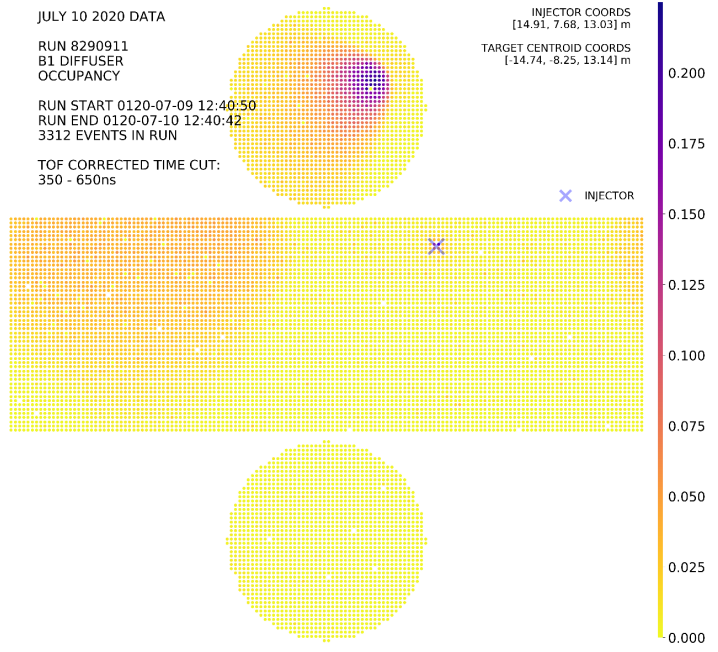
\includegraphics[width=0.49\textwidth]{Figures/B1_occupancy_diff_auto.PNG}} \hfill
    \subfloat[]{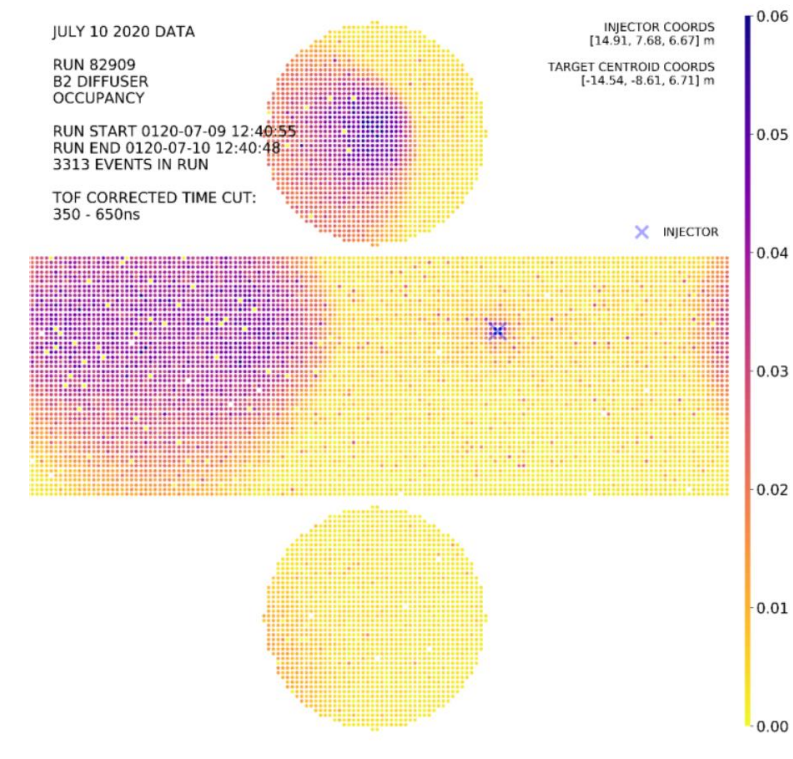
\includegraphics[width=0.49\textwidth]{Figures/B2_occupancy_diff_auto.PNG}} \par
    \subfloat[]{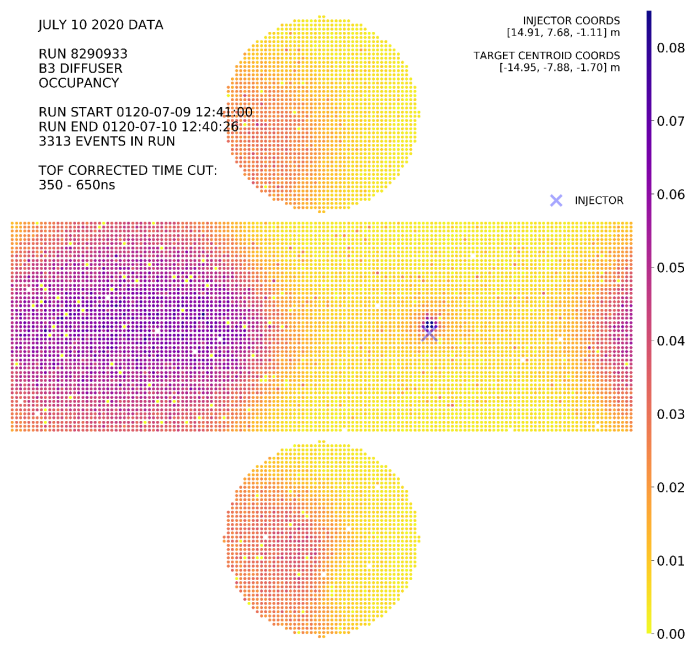
\includegraphics[width=0.49\textwidth]{Figures/B3_occupancy_diff_auto.PNG}} \hfill
    \subfloat[]{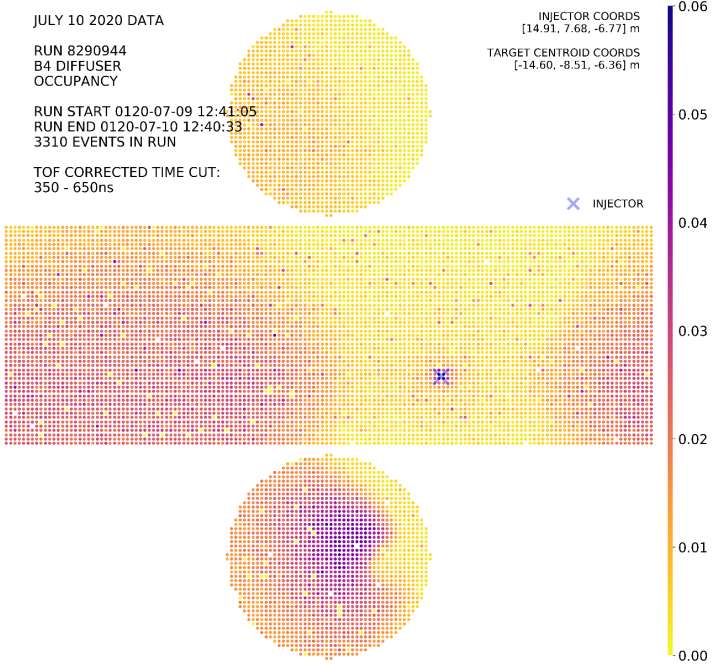
\includegraphics[width=0.49\textwidth]{Figures/B4_occupancy_diff_auto.PNG}} \par
    \subfloat[]{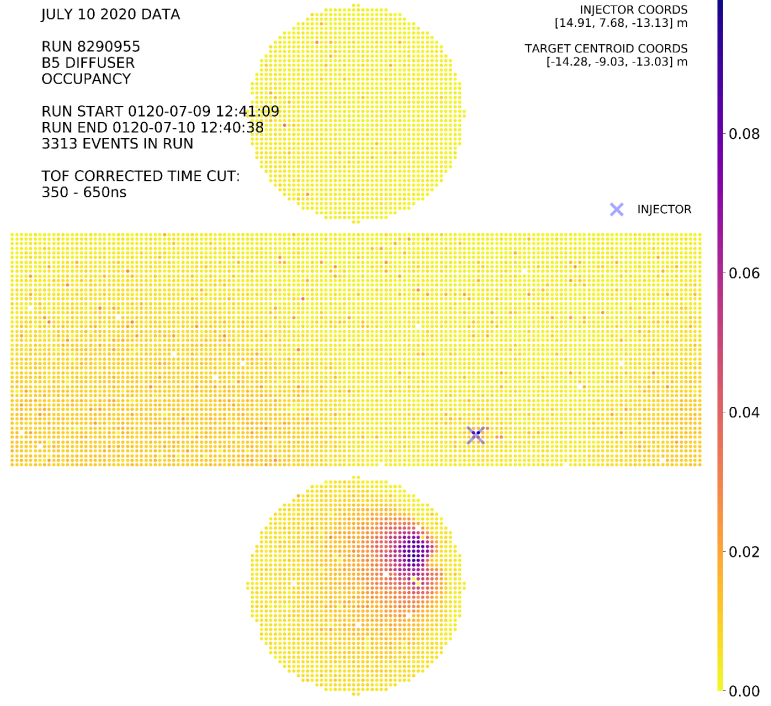
\includegraphics[width=0.49\textwidth]{Figures/B5_occupancy_diff_auto.PNG}}
    
\end{figure}


\subsubsection{Implementation of UKLI MC in SKDETSIM}
After making these fits to data the next aim was to use these light profiles as an input to SKDETSIM, the Super Kamiokande Detector Simulator. SKDETSIM uses GEANT3 (GEometry ANd Tracking 3) to simulate what the particles in each event would do inside the detector, and tracks the particle's trajectories and energy loss. Simulating the light injection from the UKLI system in SKDETSIM was done in a similar way to the Korean method of producing Monte Carlo: the same versions of the calibration scripts were used however, small modifications were made to them and to the version of SKDETSIM used to simulate the input photons from the system in the detector. The calibration scripts used for the Korean and UKLI systems both allow for the number of events and the number of injected photons to be set, in order to generate many Monte Carlo files with the absorption, Rayleigh and Mie scattering parameters. 
\newline
The first step regarding making UKLI based Monte Carlo was changing the position of the injector locations from the positions of the Korean system (shown in Table \ref{table:korean_loc}) to that of the UKLI system (shown in Table \ref{table:UKLI_loc}), due to the fact that the spacing gap rungs between the UK system and the Korean system is +70.7 cm for the B1, B2, B3 barrel injectors and -70.7 cm for the B4 and B5 injectors. The opening angle of the injectors determined by the simulation also had to be changed because the simulation had to accomodate the fact that the injectors for the UKLI system now consisted of three different opening angles for the collimator, diffuser and bare fibre optics, instead of just the bare fibre optics used in the Korean system. The way the opening angle for the Korean was set was using the``SIGBM" parameter which stands for the sigma of the input injector beam, and was produced using a Gaussian random number generator to produce the phptpn angle. However an entirely new method of determining the opening angle of the beam was needed to include the information from the light profiles taken from the test stands at Warwick. In order to understand the SIGBM parameter further however, the relationship between opening angle in degrees and SIGBM was plotted by outputting the SIGBM value and the angle to a text file during laser generation Monte Carlo production (shown in Figure \ref{fig:sigbm_angle}.)

\begin{table}[htp]
    $$
\begin{array}{|c|c|c|c|c|c|}  
    \hline \hline{\text {Korean Barrel Injector }} & {\text { x (cm)}} & {\text {y (cm)}} & {\text {z (cm)}}  \tabularnewline
    \hline \text { B1 } & 1490.73 & 768.14 & 1232.25 \\
    \hline \text { B2 } & 1490.73 & 768.14 & 595.95 \\
    \hline \text { B3 } & 1490.73 & 768.14 & -40.35 \\
    \hline \text { B4 } & 1490.73 & 768.14 & -605.95 \\
    \hline \text { B5 } & 1490.73 & 768.14 &  -1242.25 \\
    \hline \hline 
\end{array}
    $$
\caption{Barrel injector positions (x,y,z) of the Korean injectors in cm} 
\label{table:korean_loc}
\end{table}

\begin{table}[htp]
    $$
\begin{array}{|c|c|c|c|c|c|}  
    \hline \hline{\text {UKLI Barrel Injector }} & {\text { x (cm)}} & {\text {y (cm)}} & {\text {z (cm)}}  \tabularnewline
    \hline \text { B1 } & 1490.73 & 768.14 & 1302.95 \\
    \hline \text { B2 } & 1490.73 & 768.14 & 666.2 \\
    \hline \text { B3 } & 1490.73 & 768.14 & -111.05 \\
    \hline \text { B4 } & 1490.73 & 768.14 & -676.65 \\
    \hline \text { B5 } & 1490.73 & 768.14 &  -1313.95 \\
    \hline \hline 
\end{array}
    $$
\caption{Barrel injector positions (x,y,z) of the UKLI injectors in cm} 
\label{table:UKLI_loc}
\end{table}

\begin{figure}
    \centering
    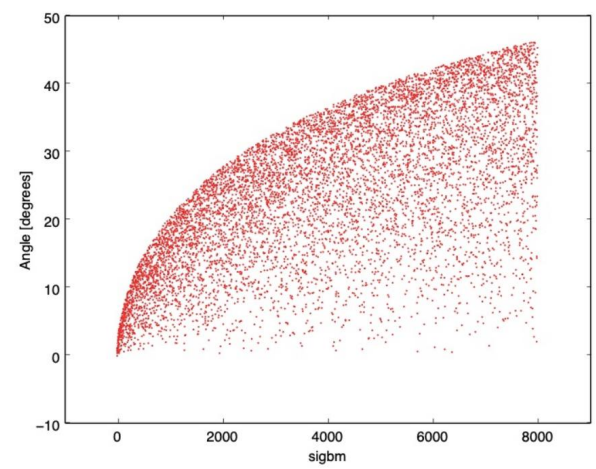
\includegraphics[width=0.7\textwidth]{Figures/sigbm_angle.png}
    \caption{Relationship between the SIGBM parameter value and the opening angle of the beam in degrees}
    \label{fig:sigbm_angle}
\end{figure}

In order to validate the positions of the targets for the UKLI system, and the relationship between the SIGBM parameter and output angle, producing charge weighted histograms from UKLI test runs is very helpful. It allows us to explore the shape of the beam profile and intensity. Figures \ref{fig:charge_weighted_nov_sept_B1} and \ref{fig:charge_weighted_nov_sept_B4} shows the charge weighted z-profiles for the September and November 2019 datasets for the B1 and B4 collimator injectors, where the blue dashed line shows the expected target position. These are produced by selecting hit PMTs which are greater than 2 m away from the injector (to avoid including PMT hits from backscattered light), and filling the histogram with the z-position of the hit PMT and the number of hits the hit PMT recieves multiplied by the corrected charge from the PMT. The corrected PMT charge is calculated using Equation \ref{eq:gain_correction}, where the gain correction value is taken from official Super-Kamiokande gain tables. 

\begin{equation}
    q/(1 + gain)
\label{eq:gain_correction}
\end{equation}

\begin{figure}
    \centering
    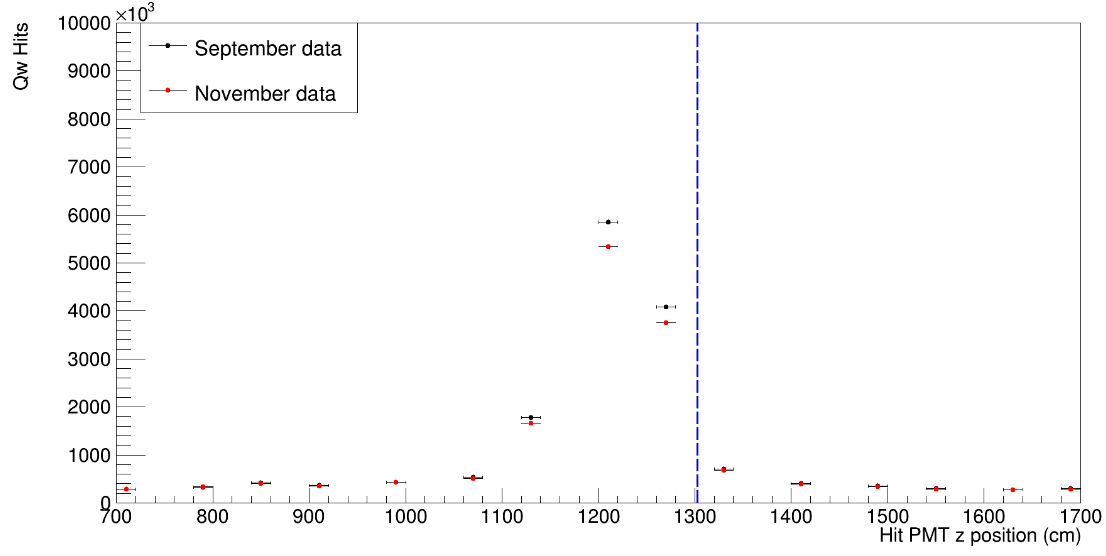
\includegraphics[width=0.9\textwidth]{Figures/charge_weighted_nov_sept_B1.PNG}
    \caption{Charge weighted z profile plots for the B1 collimator UKLI injector optic}
    \label{fig:charge_weighted_nov_sept_B1}
\end{figure}

\begin{figure}
    \centering
    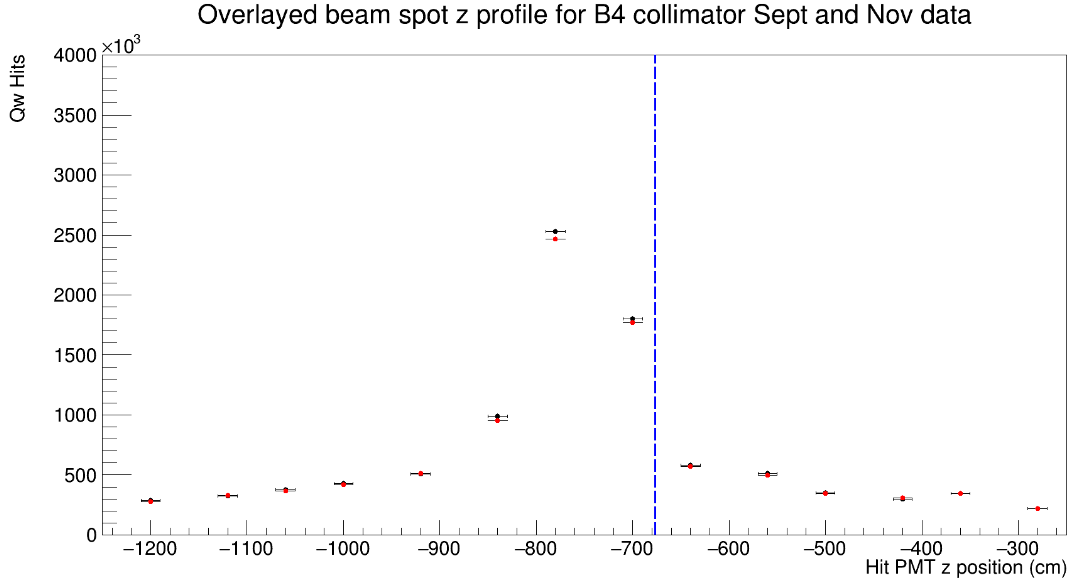
\includegraphics[width=0.9\textwidth]{Figures/charge_weighted_nov_sept_B4.PNG}
    \caption{Charge weighted z profile plots for the B4 collimator UKLI injector optic}
    \label{fig:charge_weighted_nov_sept_B4}
\end{figure}

The B1 and B4 collimator optics give the largest peaks in the charge weighted plots, while the B3 and B5 optics give the weakest peaks, practically indistinguishable from the background pedestal (even with the additional number of events taken during the November data taking runs.) The charge weighted plots were used to validate the relationship between the opening angle of the injector beam in the Monte Carlo production calibration scripts by generating Monte Carlo scripts with varying values of the SIGBM parameter (while keeping the absorption and scattering parameters the same). Fitting the charge weighted profile plots with a Gaussian and using the position of the injector target and the edge of the beam spot, the opening angle of the beam in degrees could be determined.

The width of the beam needed to be defined in order to do this however, and the standard beam radius definition is shown as in Figure \ref{fig:beam_width}. This schematic shows that the width of the beam was defined as using $1/e^2$ for the edge of the beam width, so it is taken as the point where the intensity drops to 0.135 of the Gaussian peak value. While there is good agreement at small opening angles, there is a slight discrepancy between this plot and Figure \ref{fig:sigbm_angle} at larger opening angles, where in Figure \ref{fig:sigbm_angle} the angle in degrees is consistently greater than in Figure \ref{fig:sigbm_angle_validation} for the same value of SIGBM, and this is due to SIGBM being defined as the maximum opening angle, however for small opening angles as for the collimator, the comparison is valid.

\begin{figure}
    \centering
    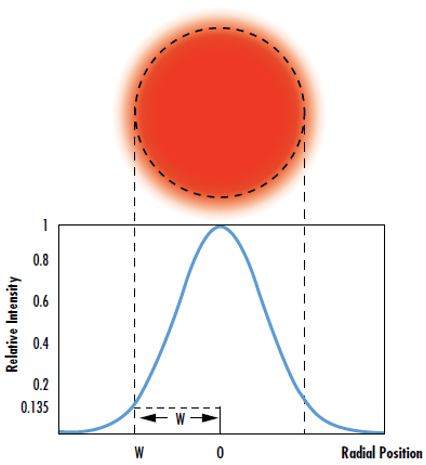
\includegraphics[width=0.7\textwidth]{Figures/beam_width.PNG}
    \caption{Schematic showing how the width of the MC beam was defined}
    \label{fig:beam_width}
\end{figure}

\begin{figure}
    \centering
    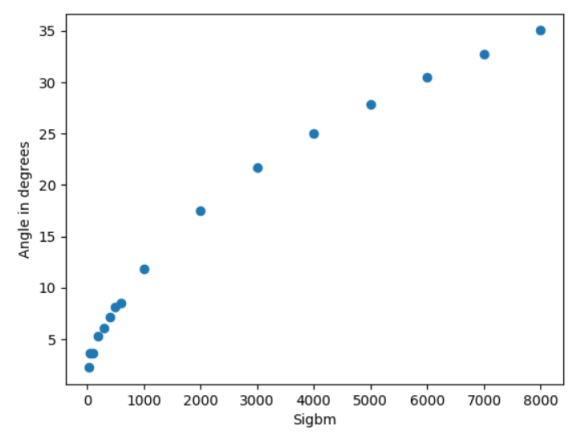
\includegraphics[width=0.7\textwidth]{Figures/sigbm_angle_validation.PNG}
    \caption{Plot of the sigbm parameter vs angle in degrees produced using calculation of the opening angle from the beam width}
    \label{fig:sigbm_angle_validation}
\end{figure}

After using the charge weighted hit plots to understand the SIGBM parameter and how the opening angle is generated by SKDETSIM more thoroughly, the next step involved using the profiles from the Warwick optic test stands (shown in Figures \ref{fig:collimator_TF1} and \ref{fig:diffuser_TF1}) in the production of this opening angle in the detector simulation. This was done by treating the profiles in Figures \ref{fig:collimator_TF1} and \ref{fig:diffuser_TF1} as Probablity Distribution Functions (PDFs) and using inverse transform sampling to make the detector simulation sample at random from it. Inverse transform sampling is a method for generating random numbers from any probability distribution by using the inverse of its cumulative distribution $F^{-1}(x)$. For continuous distributions, such as the results from the collimator and diffuser optics test stands, the algorithm for inverse transform sampling is simple. Firstly, a random variable $U$ is uniformly distributed between [0,1], and secondly the relation $X = F^{-1}_{x}(U)$ would then produce a distribution $X$ following the original probability distribution function, i.e. that of the original PDFs from the optics test stands. 

The first step is to produce the CDFs from the PDFs from the optic test stand profile tests. Figure \ref{fig:collimator_TF1} shows that the original fits to the collimator data did not reach 4 degrees, and as a result the PDFs produced needed to be linearly extrapolated from 3.5 degrees where the measurements cut off to reach 4 degrees. Figure \ref{fig:B1_PDF_CDF_coll} shows the PDFs and CDFs produced from the collimator data, and Figure \ref{fig:B1_PDF_CDF_diff} shows the PDFs and CDFs produced from the diffuser data. The CDFs are normalised with a max of one using min-max scaling. The PDFs and CDFs for the B2 - B5 collimators are shown in Figure \ref{appendix:PDF_CDF_coll} and the PDFs and CDFs for the B2 - B5 diffusers are shown in Figure \ref{appendix:PDF_CDF_diff}.


\begin{figure}
    \centering
    \label{fig:B1_PDF_CDF_coll}
    \begin{minipage}{0.45\textwidth}
        \centering
        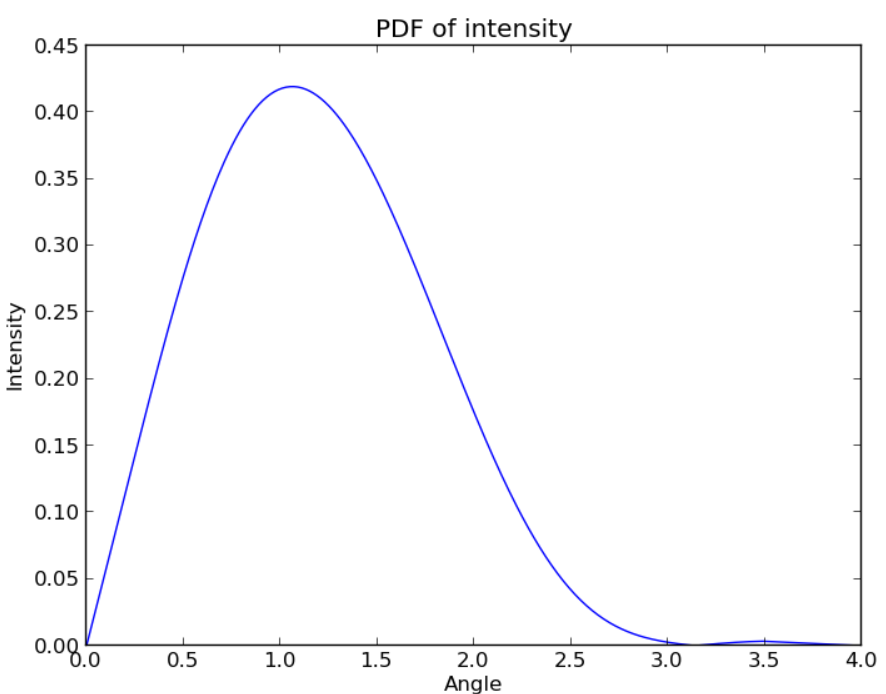
\includegraphics[width=0.9\textwidth]{Figures/B1_coll_pdf.png} % first figure itself
        \caption{PDF for the B1 collimator}
    \end{minipage}\hfill
    \begin{minipage}{0.45\textwidth}
        \centering
        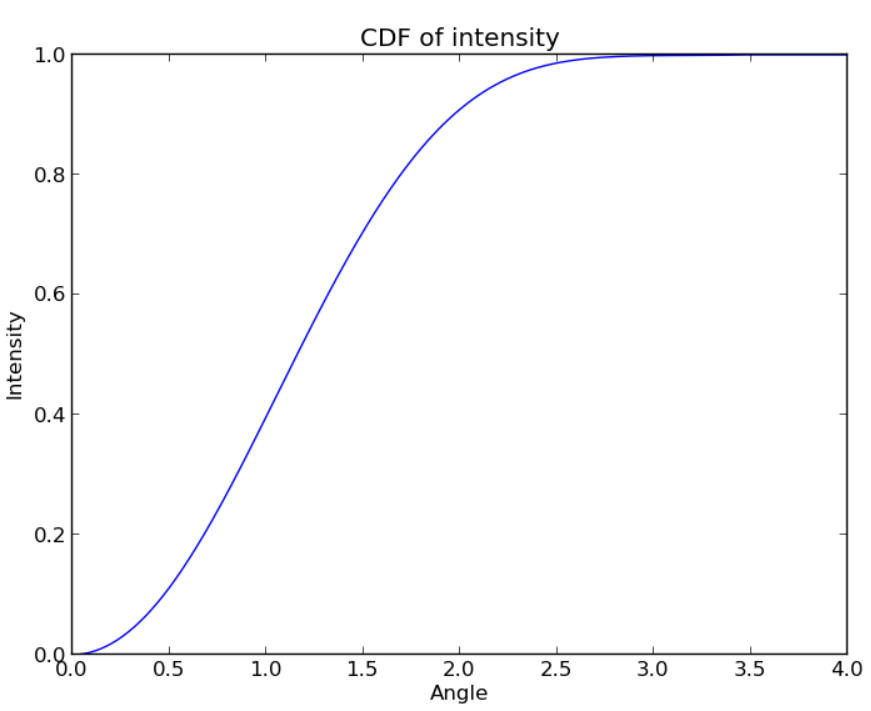
\includegraphics[width=0.9\textwidth]{Figures/B1_coll_cdf.png} % second figure itself
        \caption{CDF for the B1 collimator }
    \end{minipage}
\end{figure}

\begin{figure}
    \centering
    \label{fig:B1_PDF_CDF_diff}
    \begin{minipage}{0.45\textwidth}
        \centering
        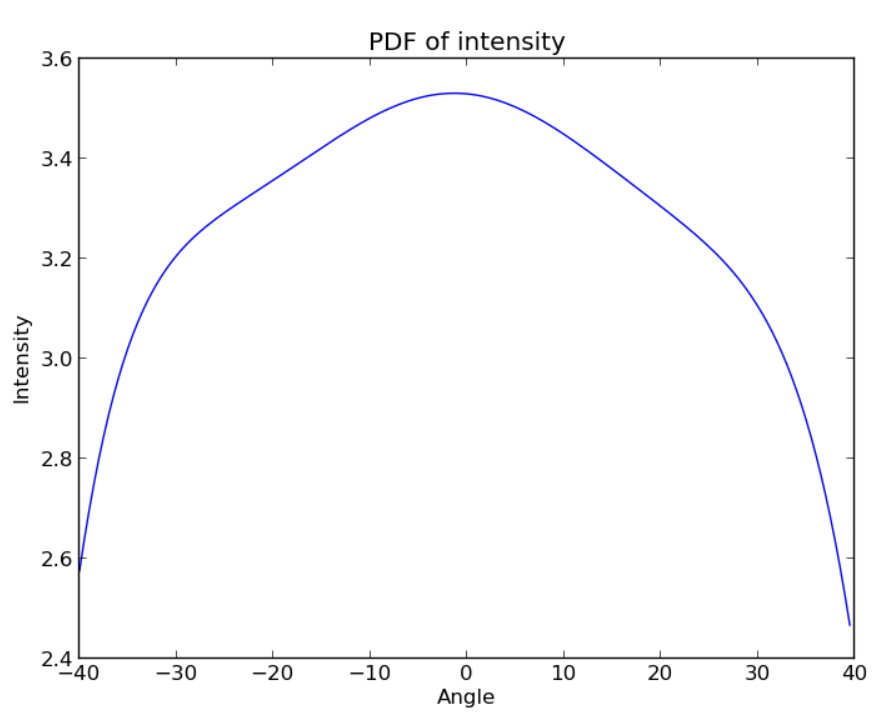
\includegraphics[width=0.9\textwidth]{Figures/B1_diff_pdf.png} % first figure itself
        \caption{PDF for the B1 diffuser}
    \end{minipage}\hfill
    \begin{minipage}{0.45\textwidth}
        \centering
        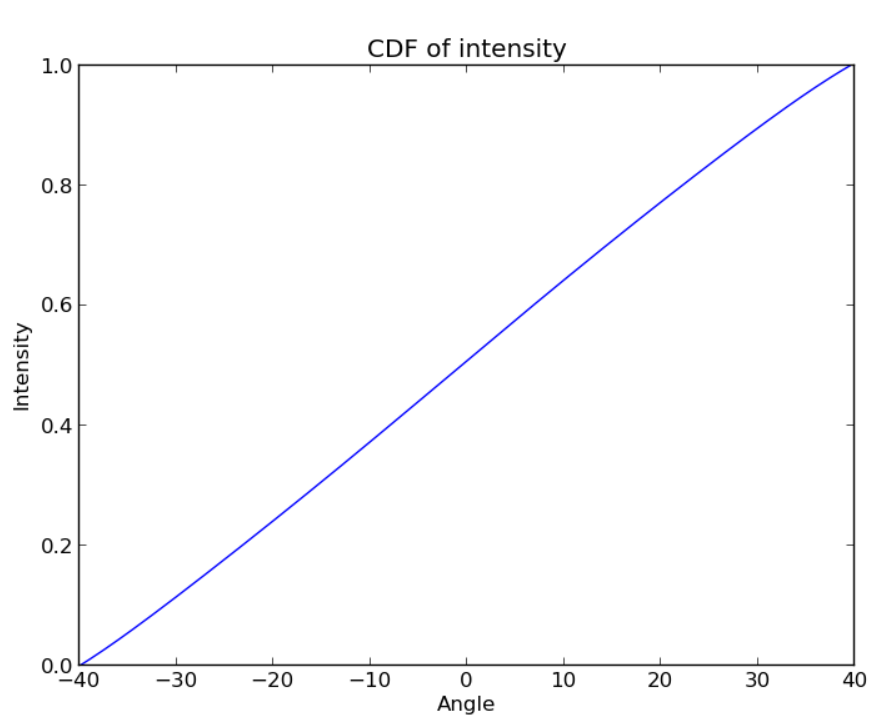
\includegraphics[width=0.9\textwidth]{Figures/B1_diff_cdf.PNG} % second figure itself
        \caption{CDF for the B1 diffuser}
    \end{minipage}
\end{figure}


After producing the normalised CDFs, the inverse of these CDFs are calculated - Figures \ref{fig:B1_PDF_CDF_inv_coll} shows the comparison of the normalised CDF data for the B1 collimator (top sublot, shown in blue) and the polynomial fit to the CDF for the B1 collimator (top subplot, shown in red), and the inverse CDF function (bottom subplot shown in green) and the polynomial fit to this inverse CDF function (bottom subplot shown in purple). Figures \ref{fig:B1_PDF_CDF_inv_diff} shows the same plot for the B1 diffuser. 

\begin{figure}
    \centering
    \begin{minipage}{0.45\textwidth}
        \centering
        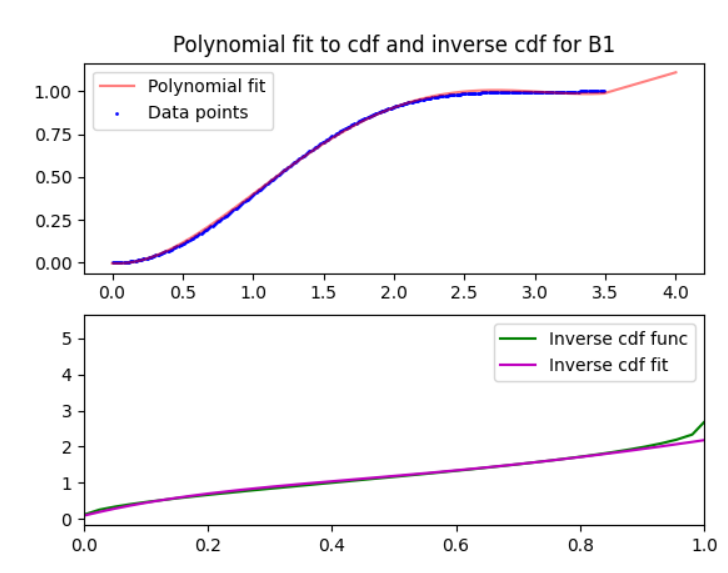
\includegraphics[width=0.9\textwidth]{Figures/B1_inv_coll_cdf.png} % first figure itself
        \caption{Inverse CDF for the B1 collimator}
        \label{fig:B1_PDF_CDF_inv_coll}
    \end{minipage}\hfill
    \begin{minipage}{0.45\textwidth}
        \centering
        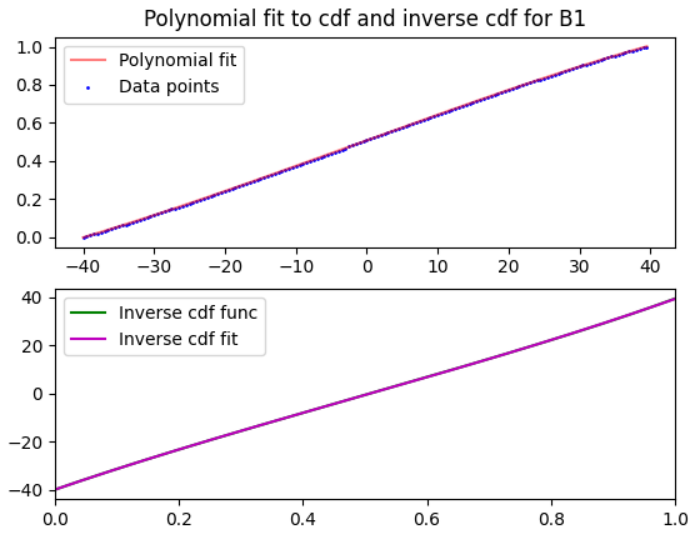
\includegraphics[width=0.9\textwidth]{Figures/B1_inv_diff_cdf.png} % second figure itself
        \caption{Inverse CDF for the B1 diffuser}
        \label{fig:B1_PDF_CDF_inv_diff}
    \end{minipage}
\end{figure}


After producing the fits to the inverse cumulative distribution functions, these funtions were inputted into the detector simulation, SKDETSIM. Removing the SIGBM parameter from the calibration scripts meant there needed to be a new way with which to generate the angle at which the photons were produced in the simulation, and this is where the inverse transform sampling occurs for the relevant fit for the selected injector and optic type. Using the same event display used to produce the occupancy plots for the autocalib data and the test run data, occupancy plots of the Monte Carlo were produced. These are shown for the B1 - B5 collimators in Figure \ref{fig:ukli_mc_coll}, and for the B1 - B5 diffusers in Figure \ref{fig:ukli_mc_diff}. These MC were produced with the abs, ray and mie parameters in the calibration scripts set to 1.0, 1.0, and 1.0 (i.e. the current detector simulation values) and the top-bottom asymmetry parameter set to 7.598, which is the most recently tuned value of this parameter. Because the original profiles from the test stands were taken in air, adjustments were made so that the refractive index of the water in the detector was taken into account when implementing the inverse CDFs into the detector simulation. 

\begin{figure}[!htbp]
    \centering
    
    \caption{Monte Carlo simulations of the B1 -B5 collimator injectors}\label{fig:ukli_mc_coll}
    
    \subfloat[]{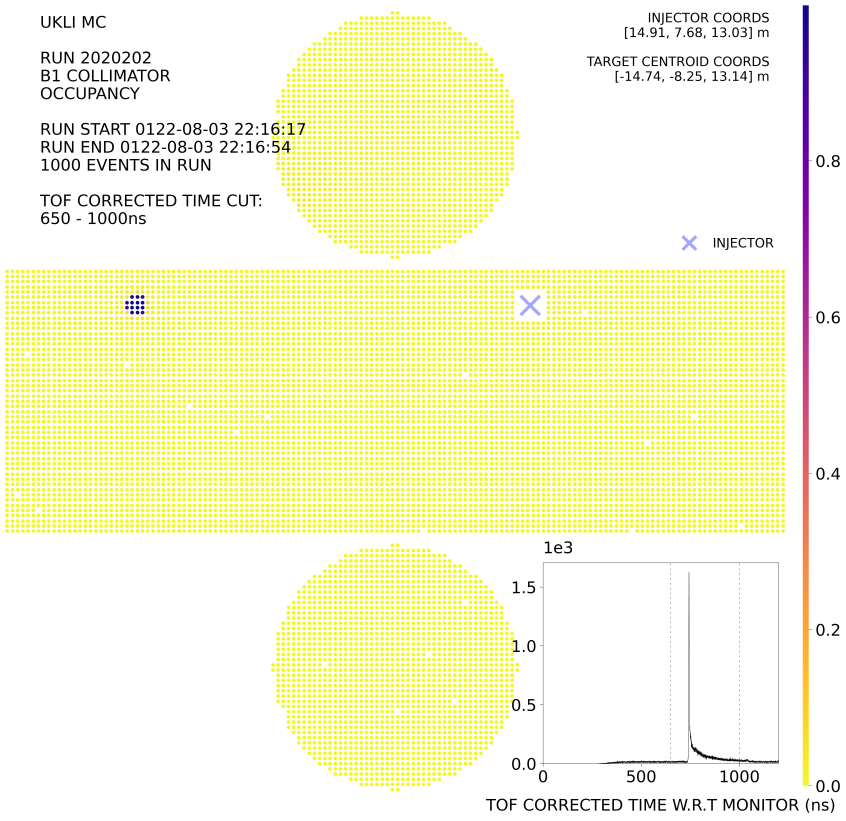
\includegraphics[width=0.33\textwidth]{Figures/ukli_mc_B1.PNG}}\hfill
    \subfloat[]{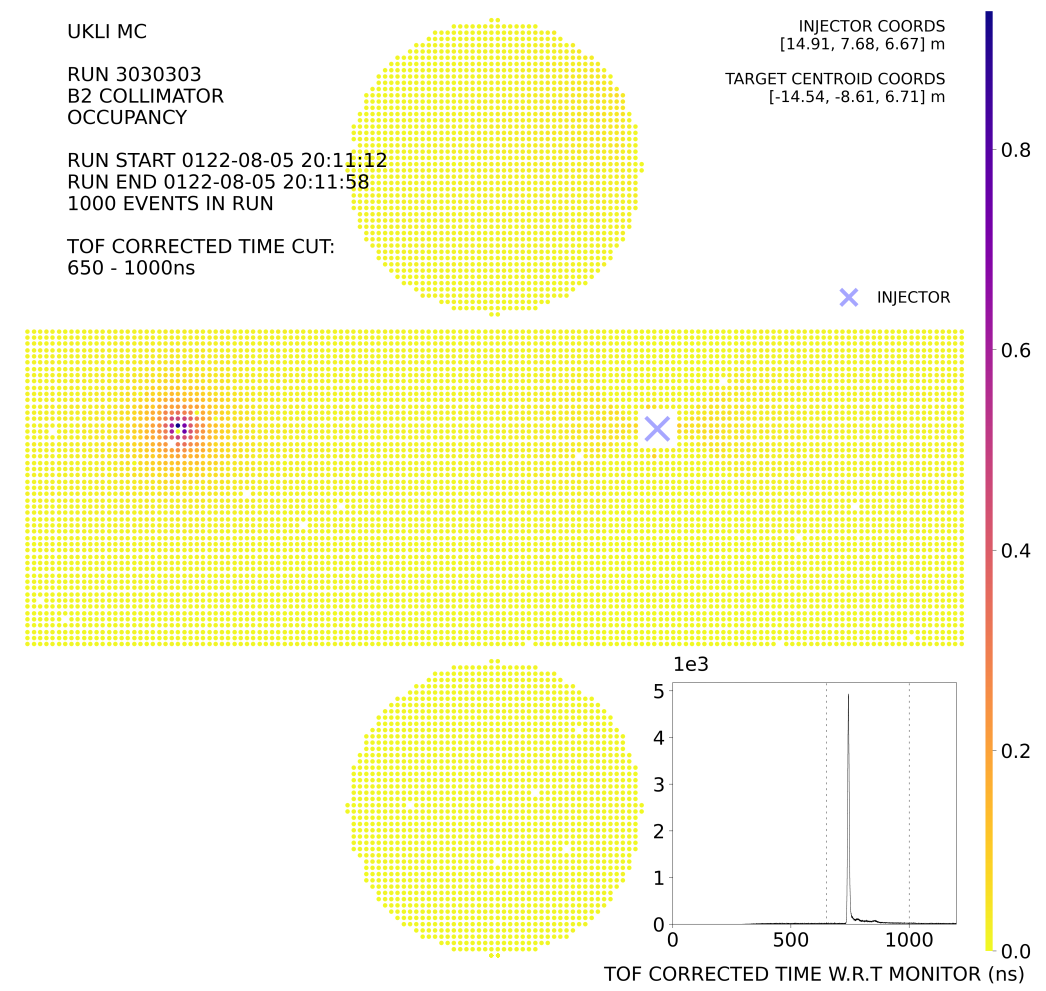
\includegraphics[width=0.33\textwidth]{Figures/ukli_mc_B2.PNG}}\hfill
    \subfloat[]{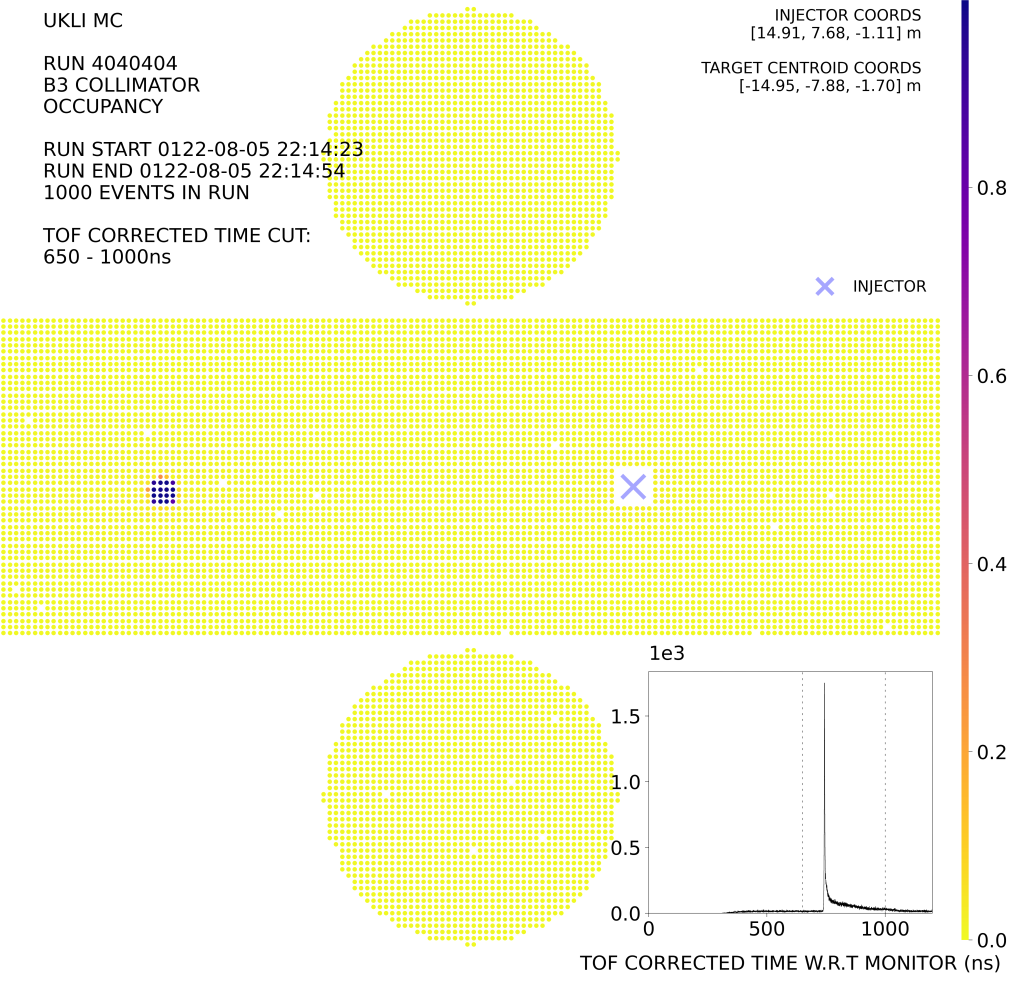
\includegraphics[width=0.33\textwidth]{Figures/ukli_mc_B3.PNG}}
    
    \subfloat[]{\includegraphics[width=0.33\textwidth]{Figures/ukli_mc_B4.PNG}}%
    \hspace*{0.005\textwidth}%
    \subfloat[]{\includegraphics[width=0.33\textwidth]{Figures/ukli_mc_B5.PNG}}
    
\end{figure}

\begin{figure}[!htbp]
    \centering
    
    \caption{Monte Carlo simulations of the B1 -B5 diffuser injectors}\label{fig:ukli_mc_diff}
    
    \subfloat[]{\includegraphics[width=0.33\textwidth]{Figures/ukli_diff_mc_B1.PNG}}\hfill
    \subfloat[]{\includegraphics[width=0.33\textwidth]{Figures/ukli_diff_mc_B2.PNG}}\hfill
    \subfloat[]{\includegraphics[width=0.33\textwidth]{Figures/ukli_diff_mc_B3.PNG}}
    
    \subfloat[]{\includegraphics[width=0.33\textwidth]{Figures/ukli_diff_mc_B4.PNG}}%
    \hspace*{0.005\textwidth}%
    \subfloat[]{\includegraphics[width=0.33\textwidth]{Figures/ukli_diff_mc_B5.PNG}}
    
\end{figure}

In order to validate the diffuser MC inverse cumulative distribution function output, a uniform distribution was run through the equation for the diffuser inverse CDF fits and the original PDF fit for each diffuser was used to fit the output points from the distribution, showing that inverse transform sampling was done correctly for the PDFs. These are shown for each diffuser in Figure \ref{fig:inv_cdf_check}. 

\begin{figure}[!htbp]
    \centering
    
    \caption{Plots of the result of running randomly sampled numbers from a uniform distibution through the inverse CDFs (in black) for each diffuser, along with the original PDF fits (in red) for the B1 - B5 diffusers.}\label{fig:inv_cdf_check}
    
    \subfloat[]{\includegraphics[width=0.33\textwidth]{Figures/inv_cdf_check_diff_B1.PNG}}\hfill
    \subfloat[]{\includegraphics[width=0.33\textwidth]{Figures/inv_cdf_check_diff_B2.PNG}}\hfill
    \subfloat[]{\includegraphics[width=0.33\textwidth]{Figures/inv_cdf_check_diff_B3.PNG}}
    
    \subfloat[]{\includegraphics[width=0.33\textwidth]{Figures/inv_cdf_check_diff_B4.PNG}}%
    \hspace*{0.005\textwidth}%
    \subfloat[]{\includegraphics[width=0.33\textwidth]{Figures/inv_cdf_check_diff_B5.PNG}}
    
\end{figure}

After producing the UKLI MC, the next step was to use them to measure the absorption and scattering parameters in a similar way to the Korean system. As mentioned earlier, this was done by producing time of flight corrected hit timing plots for UKLI MC with multiple different values of absorption, and Rayleigh and Mie scattering parameters and comparing them to the TOF corrected plots for UKLI data. Figures \ref{fig:TOF_abs}, \ref{fig:TOF_ray} and \ref{fig:TOF_mie} show the time-of-flight corrected plots for the UKLI MC B1 collimator, produced with values of the ``abs'' and ``ray'' calibration script parameter between 0.7 and 1.3 to show the affect that varying these parameters have on the time of flight corrected hits. The y-axis shows the number of hits normalised by the total charge in the detector.

\begin{figure}
    \centering
    \includegraphics[width=0.9\textwidth]{Figures/TOF_abs.PNG}
    \caption{Corrected TOF plot with varied absorption, while rayleigh and mie scattering is set to 1.0}
    \label{fig:TOF_abs}
\end{figure}

\begin{figure}
    \centering
    \includegraphics[width=0.9\textwidth]{Figures/TOF_ray.PNG}
    \caption{Corrected TOF plot with varied Rayleigh scattering, while absorption and Mie scattering is set to 1.0}
    \label{fig:TOF_ray}
\end{figure}

\begin{figure}
    \centering
    \includegraphics[width=0.9\textwidth]{Figures/TOF_mie.PNG}
    \caption{Corrected TOF plot with varied Mie scattering, while absorption and Rayleigh scattering is set to 1.0}
    \label{fig:TOF_mie}
\end{figure}

As shown in Figure \ref{fig:TOF_ray}, the TOF corrected timing plots are most affected by the Rayleigh scattering parameter, which affects the amount of hits in the scattered hits region, while varying the absorption parameter mostly affects the height of the reflected peak, as the higher the amount of absorption in the tank, the smaller the number of reflected hits. 

After producing time-of-flight corrected plots for the B1 collimator UKLI MC and overlaying it with the Run 82181 November test run data with the abs, ray, mie parameters set to 1.0, and a TBA value of 7.598, it was clear that there were disgreements between the Monte Carlo and data in both the scattered hits region and the reflected hits peak. In order to change this, the time dispersion of the reflected hits peak was varied, in order to shift the distribution and better match up the UKLI Monte Carlo and test run data. 

The time dispersion for the injected photons in the laser generation in SKDETSIM is governed by a Gaussian distributed random number generated using a Box-Muller transform, where additional time dispersion added would be the sigma of this Gaussian, and after a random number is passed through it, the output number would be added to the time for each track step of the photon giving the time dispersion.

The Box-Muller transform is a random number sampling method for making pairs of independent, normally distributed random sources from a source of uniformly distributed numbers (from between usually from between 0 and 1) \cite{10.1214/aoms/1177706645}. The form of the Box-Muller method implemented to calculate the added time dispersion is the Marsaglia polar method \cite{doi:10.1137/1006063}, which works by choosing two independent and uniformly distributed numbers (u,v) between [-1,+1], so that $s = u^{2} + v^{2}$, and if $s=0$, or $s>=1$, another pair of numbers are chosen. Then the standard normal deviate which is given by $$z_{0}=u \cdot \sqrt{\frac{-2 \ln s}{s}}$$ is multiplied by the chosen value of time dispersion in seconds and added to the mean (set to zero) to give the normally dispersed extra track step time for a photon in the distribution. 

Figure \ref{fig:gauss_time_dispersion} shows the effect of implementing this varying time dispersion on the raw hit timing output from the UKLI MC B1 collimator simulation, with the time dispersion shown for 0 ns, 5 ns, 10 ns, 15 ns, 20 ns and 100 ns. 

\begin{figure}
    \centering
    \includegraphics[width=\textwidth]{Figures/gauss_time_dispersion.PNG}
    \caption{Gaussian distributed time dispersion plots, with varying amounts of time dispersion}
    \label{fig:gauss_time_dispersion}
\end{figure}

Along with implementing the Gaussian distributed time dispersion, introducing a double gaussian for the time dispersion was also looked at, due to the height and sharpness of the reflected peak in the data being something that might be better suited to such a fit. Figure \ref{fig:double_gauss_time_dispersion} shows the raw hit timing output from the UKLI MC B1 collimator simulation with a double gaussian time dispersion, for varying time dispersion values. The x-axis on the plots show the hit time in nanoseconds, the y axis is number of events. 

\begin{figure}
    \centering
    \includegraphics[width=\textwidth]{Figures/double_gauss_time_dispersion.PNG}
    \caption{Double gaussian distributed time dispersion plots, with varying amounts of time dispersion}
    \label{fig:double_gauss_time_dispersion}
\end{figure}

Figures \ref{fig:5ns_time_dispersion}, \ref{fig:10ns_time_dispersion}, \ref{fig:15ns_time_dispersion}, \ref{fig:20ns_time_dispersion} show these time-of-flight corrected plots with both a gaussian and double gaussian time dispersion put in for varying amounts of time dispersion for 5, 10, 15 and 20 ns respectively.


\begin{figure}
    \centering
    \includegraphics[width=\textwidth]{Figures/time_dispersion_TOF_5ns.PNG}
    \caption{Gaussian and double gaussian time dispersion for 5ns for the B1 collimator TOF comparison between UKLI MC and Run 82181 test data}
    \label{fig:5ns_time_dispersion}
\end{figure}

\begin{figure}
    \centering
    \includegraphics[width=\textwidth]{Figures/time_dispersion_TOF_10ns.PNG}
    \caption{Gaussian and double gaussian time dispersion for 10ns for the B1 collimator TOF comparison between UKLI MC and Run 82181 test data}
    \label{fig:10ns_time_dispersion}
\end{figure}

\begin{figure}
    \centering
    \includegraphics[width=\textwidth]{Figures/time_dispersion_TOF_15ns.PNG}
    \caption{Gaussian and double gaussian time dispersion for 15ns for the B1 collimator TOF comparison between UKLI MC and Run 82181 test data}
    \label{fig:15ns_time_dispersion}
\end{figure}

\begin{figure}
    \centering
    \includegraphics[width=\textwidth]{Figures/time_dispersion_TOF_20ns.PNG}
    \caption{Gaussian and double gaussian time dispersion for 20ns for the B1 collimator TOF comparison between UKLI MC and Run 82181 test data}
    \label{fig:20ns_time_dispersion}
\end{figure}




For the scattered hits region (region between the dashed lines), there is now good agreement between the MC and data, with this region giving Chi2/NDF values of less than one, and the time dispersion values of 5 ns and 10 ns giving the best agreement. A problem remains regarding the reflected hits peak, where the data continues to have a much higher reflected peak than the Monte Carlo. This points to the amount of charge in the detector for the reflected peak being too large for the Monte Carlo, and further studies will be needed to be done to tune this.


\subsection{UKLI work towards Hyper-Kamiokande}

Since the first implementation of the UKLI MC, there have been several improvements made to the diffuser profiles, with a full 2$\pi$ diffuser profile produced from UKLI diffusers placed in a test stand in Sheffield. There were two types of diffusers involved in creating the 2D profiles: the ``D5'' diffuser (and SK install spare diffuser) and ``HP1'', a prototype for Hyper-Kamiokande. Profile measurements for the diffusers were made in both air and water, and Figure \ref{fig:diffuser_tank_sheff} shows the test stand setup at Sheffield, along with Figure \ref{fig:D5_diffuser} and Figure \ref{fig:HP1_diffuser} which show the D5 and HP1 diffusers respectively.


\begin{figure}
    \centering
     \begin{subfigure}[b]{0.9\linewidth}
      \includegraphics[width=\linewidth]{Figures/diffuser_tank_sheff.PNG}
      \caption{Diffuser tank setup at Sheffield}
      \label{fig:diffuser_tank_sheff} 
     \end{subfigure}
     \begin{subfigure}[b]{0.3\linewidth}
       \includegraphics[width=\linewidth]{Figures/D5_diffuser.PNG}
        \caption{D5 (SK spare) diffuser} 
     \label{fig:D5_diffuser}
      \end{subfigure} \hfill%
      \begin{subfigure}[b]{0.3\linewidth}
      \includegraphics[width=\linewidth]{Figures/HP1_diffuser.PNG}
      \caption{HP1 (HK protoype) diffuser}
      \label{fig:HP1_diffuser}
      \end{subfigure}
\end{figure}

In Figure \ref{fig:diffuser_tank_sheff}, not only is there a $\theta$ rotational stand about the vertical axis, there is also $\phi$ rotation about a horzontal axis, allowing for a 2D profile instead of the 1D profiles produced by the Warwick test stand previously. Figure \ref{fig:D5_sheff_2D_air} and Figure \ref{fig:D5_sheff_2D_water} show the 2D profiles for the D5 diffuser produced in air and water, with the $\theta$ and $\phi$ rotations labelled. 


\begin{figure}
    \centering
     \begin{subfigure}[b]{0.45\linewidth}
      \includegraphics[width=\linewidth]{Figures/D5_sheff_2D_air.PNG}
      \caption{2D profile for the D5 diffuser in air}
      \label{fig:D5_sheff_2D_air} 
     \end{subfigure}
     \begin{subfigure}[b]{0.45\linewidth}
       \includegraphics[width=\linewidth]{Figures/D5_sheff_2D_water.PNG}
        \caption{2D profile for the D5 diffuser in water} 
     \label{fig:D5_sheff_2D_water}
      \end{subfigure} 
\end{figure}

To investigate the relationship between polar angle, azimuthal angle and the amplitude of the light, plots were made for the D5 and HP1 diffusers of the variation of amplitude vs polar angle, for measurements of azimuthal angle in 30$\degree$ intervals. This would give an indication of how uniform the profile is by seeing how closely the values of amplitude for each azimuthal angle are to each other. This is shown in Figure \ref{fig:HP1_D5_azimuthal}, along with the coefficient of quartile variation (CQV) of the amplitude, to show the spread of the data and used instead of the standard deviation as a more robust measure as it will not be affected by outliers.  This data is shown for both the D5 and HP1 diffusers in air and also water, with three distinct regions (shown by the dashed lines) across which the amplitude varies most. 

\begin{figure}[!htbp]
    \centering
    
    \caption{Amplitude and Amplitude CQV plotted against polar angle (in degrees) for different values of azimuthal angle in air and water for the D5 and HP1 diffusers}\label{fig:HP1_D5_azimuthal}
    
    \subfloat[]{\includegraphics[width=0.45\textwidth]{Figures/cqv_D5_air.PNG}}
    \subfloat[]{\includegraphics[width=0.45\textwidth]{Figures/cqv_D5_water.PNG}}\\
    \subfloat[]{\includegraphics[width=0.45\textwidth]{Figures/CQV_HP1_air.PNG}}
    \subfloat[]{\includegraphics[width=0.45\textwidth]{Figures/CQV_hp1_water}}%
    
\end{figure}

The reason for the largest CQV values for the larger values of polar angle is due to smaller amplitude values showing more variation than for larger amplitude values if there an inherent systematic variation stemming from measurement apparatus or dark noise in the tank. 

To conclude, initial 1D light profiles for the collimator and diffuser optics from the test stand at Warwick have been put into the detector simulation and inverse transform sampling has been used to generate the output angle of the outgoing photon according to the input light profile shape. This has been validated by occupancy plots and also running uniformly generated random numbers through the inverse cumulative distribution function to produce the input profile probability distribution function. In addition to this, by generating time-of-flight corrected hit time distributions, the timing region which shows the scattered hits has been adjusted to match up with test run data, by understanding how to tweak the amount of timing dispersion to have different distributions. Future work in order to implement 2D profiles have been started with the help from colleagues at Sheffield, and scans and fits to the polar and azimuthal angle have been made. 

